% =====================================================================================================
%  Project report - DSDR recloser-fuse coordination, IEEE 13-node feeder, DIgSILENT PowerFactory
%  Generated by make_report_latex.py from report_template.tex: edit the TEMPLATE, not main.tex,
%  if you want the tables to stay linked to the results.  Compile with pdfLaTeX, twice.
% =====================================================================================================
\documentclass[12pt,letterpaper]{article}

\usepackage[T1]{fontenc}
\usepackage[utf8]{inputenc}
\usepackage{mathptmx}                       % Times, as in the reference report
\usepackage[left=1.2in,right=1in,top=1in,bottom=1in]{geometry}
\usepackage{setspace}
\usepackage{amsmath,amssymb}
\usepackage{graphicx}
\usepackage{booktabs,array,tabularx,longtable,multirow}
\usepackage[table]{xcolor}
\usepackage{float}
\usepackage{enumitem}
\usepackage{titlesec}
\usepackage[font=small,labelfont=bf,labelsep=colon]{caption}
\usepackage[hidelinks]{hyperref}

\graphicspath{{figures/}{./}}
% a picture that has not been uploaded gives a framed note instead of stopping the compilation
\let\OrigIncludegraphics\includegraphics
\renewcommand{\includegraphics}[2][]{%
  \IfFileExists{#2}{\OrigIncludegraphics[#1]{#2}}{%
  \IfFileExists{figures/#2}{\OrigIncludegraphics[#1]{figures/#2}}{%
  \IfFileExists{report_pictures.pdf}{\OrigIncludegraphics[#1,page=\csname pic@#2\endcsname]{report_pictures.pdf}}{%
  \fbox{\parbox{0.6\linewidth}{\centering\small picture \texttt{\detokenize{#2}} not uploaded yet}}}}}}
% page of each picture in report_pictures.pdf (all pictures in one file)
\expandafter\def\csname pic@case05.png\endcsname{1}
\expandafter\def\csname pic@case07.png\endcsname{2}
\expandafter\def\csname pic@cd_sequence.png\endcsname{3}
\expandafter\def\csname pic@cd_summary.png\endcsname{4}
\expandafter\def\csname pic@fig01.png\endcsname{5}
\expandafter\def\csname pic@fig03.png\endcsname{6}
\expandafter\def\csname pic@fig08.png\endcsname{7}
\expandafter\def\csname pic@fig09.png\endcsname{8}
\expandafter\def\csname pic@fig10.png\endcsname{9}
\expandafter\def\csname pic@fig11.png\endcsname{10}
\expandafter\def\csname pic@fig12.png\endcsname{11}
\expandafter\def\csname pic@fig13.png\endcsname{12}
\expandafter\def\csname pic@fig14.png\endcsname{13}
\expandafter\def\csname pic@fig15.png\endcsname{14}
\expandafter\def\csname pic@fig16.png\endcsname{15}
\expandafter\def\csname pic@fig17.png\endcsname{16}
\expandafter\def\csname pic@flowchart.png\endcsname{17}
\expandafter\def\csname pic@sld.png\endcsname{18}
\expandafter\def\csname pic@tu_logo.png\endcsname{19}
\onehalfspacing
\setlength{\parindent}{0pt}
\setlength{\parskip}{8pt}
\tolerance=1000
\emergencystretch=3em
\hbadness=5000
\setlist{itemsep=2pt,topsep=2pt}
\renewcommand{\arraystretch}{1.15}

% ---- headings: "CHAPTER ONE: INTRODUCTION", then 1.1, 1.1.1 -------------------------------------------
\newcounter{chap}
\makeatletter\@addtoreset{subsection}{chap}\makeatother
\renewcommand{\thesubsection}{\arabic{chap}.\arabic{subsection}}
\renewcommand{\thesubsubsection}{\thesubsection.\arabic{subsubsection}}
\titleformat{\section}[block]{\normalfont\bfseries\Large\centering}{}{0pt}{}
\titlespacing*{\section}{0pt}{0pt}{14pt}
\titleformat{\subsection}{\normalfont\bfseries\large}{\thesubsection}{0.6em}{}
\titlespacing*{\subsection}{0pt}{12pt}{4pt}
\titleformat{\subsubsection}{\normalfont\bfseries\normalsize}{\thesubsubsection}{0.6em}{}
\titlespacing*{\subsubsection}{0pt}{8pt}{2pt}
\setcounter{secnumdepth}{3}
\setcounter{tocdepth}{3}

% \chapterhead{ONE}{INTRODUCTION}
\newcommand{\chapterhead}[2]{\clearpage\refstepcounter{chap}\phantomsection
  \section*{CHAPTER #1: #2}\addcontentsline{toc}{section}{CHAPTER #1: #2}}
% \fronthead{ABSTRACT}  /  \appendixhead{A}{TITLE}
\newcommand{\fronthead}[1]{\clearpage\phantomsection\section*{#1}\addcontentsline{toc}{section}{#1}}
\newcommand{\appendixhead}[2]{\clearpage\phantomsection
  \section*{APPENDIX #1: #2}\addcontentsline{toc}{section}{APPENDIX #1: #2}}

\renewcommand{\contentsname}{TABLE OF CONTENTS}
\renewcommand{\listfigurename}{LIST OF FIGURES}
\renewcommand{\listtablename}{LIST OF TABLES}
\renewcommand{\refname}{REFERENCES}

% ---- table helpers ---------------------------------------------------------------------------------
\definecolor{okc}{HTML}{DFF3DF}
\definecolor{noc}{HTML}{FBE0E0}
\definecolor{headc}{HTML}{E6ECF5}
\newcommand{\ok}{\cellcolor{okc}$\checkmark$}
\newcommand{\no}{\cellcolor{noc}$\times$}
\newcommand{\hd}{\rowcolor{headc}}
\newcolumntype{L}{>{\raggedright\arraybackslash}X}
\newcommand{\ohm}{\,\ensuremath{\Omega}}
\newcommand{\PF}{PowerFactory}

\begin{document}

% =====================================================================================================
%  TITLE PAGE
% =====================================================================================================
\begin{titlepage}
\centering
{\large\bfseries TRIBHUVAN UNIVERSITY\par}
{\bfseries INSTITUTE OF ENGINEERING\par}
{\bfseries PULCHOWK CAMPUS\par}
\vspace{1.0cm}

\includegraphics[width=3.4cm]{tu_logo.png}\par
\vspace{1.2cm}
{\bfseries PROJECT REPORT\par}
{\itshape on\par}
\vspace{0.4cm}
{\large\bfseries An Adaptive Overcurrent Protection Scheme for\\
Dual-Setting Directional Recloser and Fuse Coordination\\
in Unbalanced Distribution Networks With Distributed Generation\par}
\vspace{1.0cm}
{\bfseries Submitted by\par}
{\bfseries Jhala Nath Kafle\par}
Roll No. 081MSPSE009\par
\vspace{1.4cm}
{\small\itshape A report submitted in partial fulfillment of the requirements for the 3rd semester project of the
Master's Degree in Power System Engineering\par}
\vfill
Department of Electrical Engineering\par
October 2026\par
\end{titlepage}
\setcounter{page}{2}

% =====================================================================================================
\fronthead{ACKNOWLEDGEMENT}
% EDIT: add the names of the supervisor and of anyone else to be thanked.
I express my sincere gratitude to my project supervisor and to the Department of Electrical Engineering,
Pulchowk Campus, Institute of Engineering, for their guidance, for the review comments on the earlier
progress report, and for the facilities that made this work possible. I also thank my colleagues of the
M.Sc.\ Power System Engineering programme for the discussions on distribution protection and on the use of
DIgSILENT \PF.

% =====================================================================================================
\fronthead{ABSTRACT}
Distributed generation (DG) changes the magnitude and the direction of the fault current in medium-voltage
distribution feeders and can therefore invalidate a conventional, fixed-setting recloser--fuse coordination.
This project independently implements and evaluates the dual-setting directional recloser (DSDR) method of
Yousaf \textit{et al.} on the IEEE 13-node test feeder. The earlier phase of the project used
MATLAB/Simulink; the complete study has now been rebuilt in \textbf{DIgSILENT \PF{} 2021}, driven by Python
scripts, so that every table and figure is regenerated from the model by one command.

The model uses the feeder of the DIgSILENT example library with the 115/4.16\,kV substation transformer, a
4.05\,MVA synchronous DG at node 692 with the full machine data of the reference paper, the manufacturer
curves of the two reclosers (GE IAC77B801A and GE/Alstom CDG34) and library fuse curves (Gould-Shawmut
A055C). Unbalanced load flow, short-circuit calculation for all fault types and phase combinations, and an
electromagnetic-transient (EMT) simulation of the reclosing sequence were carried out.

The rated branch currents agree with the reference paper within 2\,\%. The fault levels follow the IEEE
short-circuit benchmark and are lower than the values printed in the paper, by 4 to 60\,\% on the feeder
branches. Without DG the
scheme is coordinated in all 39 node/fault-type cells. With the DG and a conventional single-setting
recloser R2, coordination is held in only 24 of 39 cells; 29 cells agree with
the paper's Fig.~14. With R2 as a DSDR and the fuse revision of the method, coordination is held in
38 of 39 cells. With the same fuses and a single-setting R2 only 31 cells are
held, so the dual setting itself restores seven cells. One cell (line-to-ground fault at 692) cannot be
restored with the available dial range, and faults downstream of R2 remain fed directly by the DG.
\PF's own relay and fuse models confirm the calculated operating times within 1.22\,\% over
1896 operating times.

The report documents the model, the settings, the results, the differences from the reference paper and
their causes, and the work that remains: the extension to the IEEE 34-node feeder.

\textbf{Keywords:} distributed generation, dual-setting directional recloser, fuse saving, recloser--fuse
coordination, IEEE 13-node feeder, DIgSILENT \PF.

% =====================================================================================================
\clearpage
\begin{spacing}{1.1}
\tableofcontents
\clearpage
\phantomsection\addcontentsline{toc}{section}{LIST OF FIGURES}
\listoffigures
\clearpage
\phantomsection\addcontentsline{toc}{section}{LIST OF TABLES}
\listoftables
\end{spacing}

% =====================================================================================================
\fronthead{LIST OF ABBREVIATIONS}
\begin{center}
\begin{tabular}{@{}ll@{}}
\toprule
\textbf{Abbreviation} & \textbf{Meaning} \\
\midrule
CT & Current Transformer \\
CTI & Coordination Time Interval \\
DG & Distributed Generation \\
DSDR & Dual-Setting Directional Recloser \\
EMT & Electromagnetic Transient (simulation) \\
LG & Line-to-Ground fault \\
LL & Line-to-Line fault \\
LLG & Line-to-Line-to-Ground fault \\
LLL & Three-Phase fault \\
MMT & Minimum Melting Time \\
OLF & Overload Factor \\
PD & Protection Device \\
PF & DIgSILENT PowerFactory \\
R1 & Feeder-Head Recloser \\
R2 & Mid-Line Recloser (the DSDR) \\
RMS & Root Mean Square \\
SBDG & Synchronous-Based Distributed Generator \\
TCC & Time-Current Characteristic \\
TCT & Total Clearing Time \\
TDS & Time Dial Setting \\
TMS & Time Multiplier Setting \\
\bottomrule
\end{tabular}
\end{center}

\fronthead{LIST OF SYMBOLS}
\begin{center}
\begin{tabular}{@{}ll@{}}
\toprule
\textbf{Symbol} & \textbf{Description} \\
\midrule
$I_f$ & Fault current seen by a protection device \\
$I_p$ & Pickup current of a recloser \\
$I_s$ & Plug (current) setting of the CDG relay \\
$I_{nom}$ & Rated (load) current \\
$M$ & Multiple of pickup, $I_f/I_p$ \\
$TDS$, $TMS$ & Time-dial / time-multiplier setting \\
$t_F$, $t_D$ & Fast and delayed operating time of a recloser \\
$t_{MMT}$, $t_{TCT}$ & Minimum-melting and total-clearing time of a fuse \\
$A$, $B$, $n$ & Constants of the inverse-time curve \\
$a_i$, $b_i$ & Coefficients of the fuse characteristic \\
$k$, $l$, $m$ & Index of the recloser, of a downstream and of an upstream fault location \\
$z$, $i$ & Number of series fuses in the fault path; position of a fuse in it \\
$Z_f$ & Fault impedance \\
$X_d$, $X'_d$, $X''_d$ & Direct-axis synchronous, transient and subtransient reactance \\
$X_q$, $X'_q$, $X''_q$ & Quadrature-axis reactances \\
$R_a$ & Armature resistance \\
\bottomrule
\end{tabular}
\end{center}

% =====================================================================================================
\chapterhead{ONE}{INTRODUCTION}

\subsection{Background}
Overcurrent protection of radial distribution networks is traditionally coordinated on the assumption that
the fault current flows from the substation towards the loads. A recloser upstream of a fuse first operates on
a fast characteristic, to clear a temporary fault before the fuse melts, and then on a delayed
characteristic, to let the fuse clear a permanent fault. This \emph{fuse-saving} arrangement only works while
the fuse curve lies between the two recloser curves over the whole range of fault currents.

Distributed generation changes this. A DG downstream of a recloser feeds current towards a fault upstream of
it, so the recloser carries current in the reverse direction, and a fuse between the two sources carries the
sum of both contributions while each recloser carries only one. The current seen by a protection device then
depends on the fault location, the topology and the DG, and a single fixed setting is no longer suitable for
both directions.

The dual-setting directional recloser (DSDR) addresses this by giving the mid-line recloser separate pickup
and time-dial settings for the forward and for the reverse direction. This project implements the method of
Yousaf \textit{et al.}~\cite{yousaf2022} on the IEEE 13-node feeder in DIgSILENT \PF{} and evaluates it.

\subsection{Problem Statement}
The problem addressed is the loss of recloser--fuse coordination caused by the change of fault-current
magnitude and direction when a DG is connected. A conventional scheme that is coordinated without DG may lose
the fuse-saving property in the zone between the grid and the DG. The project investigates whether the DSDR
method restores the coordination when it is reproduced with an independently built model and with the real
characteristics of the devices named in the paper.

\subsection{Objectives}
\subsubsection{General Objective}
To build and validate a DIgSILENT \PF{} implementation of the DSDR protection-coordination method on the IEEE
13-node test feeder, with and without distributed generation, and to compare the results with the reference
paper.

\subsubsection{Specific Objectives}
\begin{enumerate}
\item Build and verify the IEEE 13-node feeder with the protection devices of the reference paper and compare
      the branch currents with its Table~II.
\item Perform unbalanced load-flow and short-circuit studies for all fault types and phase combinations.
\item Calculate the recloser pickup currents, time dials and the fuse coefficients with the paper's equations.
\item Establish the conventional recloser--fuse coordination without DG.
\item Connect the 4.05\,MVA synchronous DG at node 692 and quantify the change of the fault currents and of
      their direction at the reclosers.
\item Classify the coordination with DG for a conventional recloser R2 (Fig.~14 of the paper).
\item Design the forward and reverse settings of R2 as a DSDR and classify the coordination again
      (Fig.~17 and Table~IV of the paper).
\item Verify the reclosing sequence in the time domain (Fig.~10 of the paper).
\item Identify and explain every difference from the reference paper.
\end{enumerate}

\subsection{Scope of the Study}
The study covers the IEEE 13-node feeder: unbalanced load flow, LG, LL, LLG and LLL faults at twelve fault
locations, pickup and time-dial calculation, fuse coordination, the DSDR forward and reverse settings, the
coordination classification with and without the DSDR, and one EMT simulation. The IEEE 34-node part of
the paper is outside the completed work.

\subsection{Significance of the Study}
The study gives a reproducible implementation of a protection-coordination method for feeders with DG in a
tool that utilities use. It shows what the method achieves when the real relay dials and fuse sizes are
respected, and it separates the contribution of the dual setting from the contribution of the fuse revision,
which the paper does not do.

\subsection{Limitations of the Study}
\begin{itemize}
\item The paper does not print the settings of R2, the fuse sizes behind its Table~IV, the source impedance,
      or the fault type of each row of Table~IV. These had to be chosen; every choice and its basis is listed
      in Section~\ref{sec:assumptions}.
\item The library model of the CDG34 relay is not directional. The two setting groups are modelled as
      separate relay units and the direction is assigned from the fault location.
\item Coordination is judged with a zero-margin criterion (the fuse must not start to melt before the fast
      trip). Section~\ref{sec:margin} shows how the result changes with a breaker time and a fuse margin.
\item Fig.~7 of the paper (CTI against DG penetration) is not reproduced, because the paper does not define
      the quantity it plots.
\item The IEEE 34-node feeder has not been modelled.
\end{itemize}

\subsection{Organization of the Report}
Chapter One introduces the problem and the objectives. Chapter Two reviews the protection concepts and the
reference paper. Chapter Three gives the method and its equations. Chapter Four describes the \PF{} model,
the DG, the protection devices and the simulation cases. Chapter Five presents the results. Chapter Six
compares them with the reference paper. Chapter Seven discusses the findings and their limits. Chapter Eight
gives the conclusions and the remaining work.

% =====================================================================================================
\chapterhead{TWO}{LITERATURE REVIEW AND REFERENCE PAPER}

\subsection{Overview of Overcurrent Protection}
An overcurrent device operates when the current exceeds its pickup. With an inverse-time characteristic the
operating time falls as the multiple of pickup rises, so a device close to the fault clears it quickly while
upstream devices act later as backup~\cite{benmouyal1999}.

\subsection{Distribution Network Protection}
Distribution feeders combine reclosers and fuses. A recloser distinguishes temporary from permanent faults by
its fast and delayed operations; a fuse isolates a permanent fault on a lateral.

\subsection{Overcurrent Relays}
The pickup setting fixes the current above which the inverse-time characteristic is active. The time dial
scales the operating time without changing the shape of the curve. Real relays offer discrete taps and a
limited dial range, which is decisive in this study.

\subsection{Directional Overcurrent Relays}
A directional element compares the current with a polarising voltage and so distinguishes the direction of
the fault. It becomes necessary when a DG makes the fault current flow from the feeder towards the
substation.

\subsection{Fuse--Recloser Coordination}
For fuse saving the fast recloser curve must lie below the minimum-melting curve of the fuse, and the delayed
curve above its total-clearing curve. Fuses in series are coordinated with the 75\,\% rule: the downstream
fuse must clear within 75\,\% of the melting time of the upstream fuse. Figure~
ef{fig:f1} shows the
principle with the curves of the model.

\begin{figure}[H]
\centering
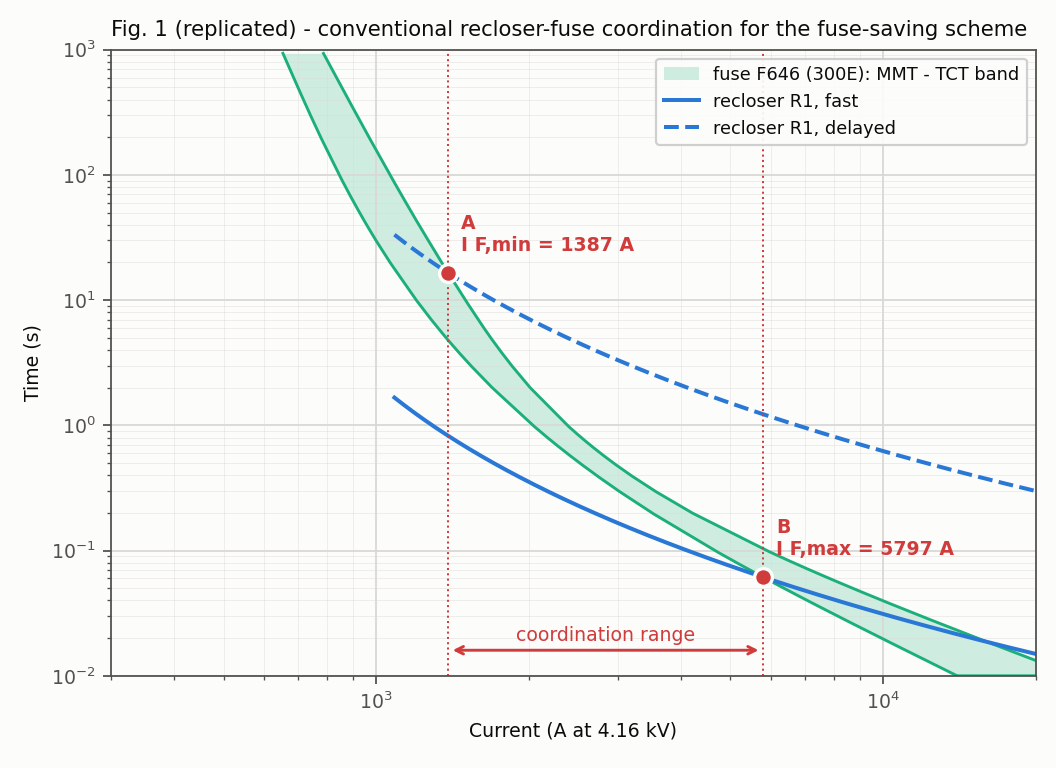
\includegraphics[width=0.72\textwidth]{fig01.png}
\caption{Conventional recloser--fuse coordination: fast and delayed curve of R1 around the band of fuse F646.
Coordination holds between the two crossing currents.}
\label{fig:f1}
\end{figure}

\subsection{Impact of Distributed Generation on Protection Coordination}
A DG raises the current through the fuses and can reverse the current through a recloser. The recloser and
the fuse then no longer carry the same current, and a setting that was coordinated without DG may let the fuse
melt before the fast trip~\cite{naiem2012}.

\subsection{Adaptive Protection}
Adaptive protection changes the settings with the state of the network. In the DSDR the device holds two
setting groups and selects one from the direction of the fault current, so no communication is needed.

\subsection{Protection of Unbalanced Distribution Networks}
The IEEE 13-node feeder~\cite{kersting1991} has single-phase, two-phase and three-phase sections and
unbalanced loads. The calculations must therefore keep the phases that really exist at each node and be made
per phase.

\subsection{Review of Related Research}
Naiem \textit{et al.}~\cite{naiem2012} classify whether recloser--fuse coordination exists for each fault
with DG. Yousaf \textit{et al.}~\cite{yousaf2020} give a benchmark overcurrent protection scheme, with
device types and fuse sizes, for the IEEE 13-node feeder; the present work takes the fuse sizes that the
reference paper does not show from that source. Kersting and Shirek~\cite{kersting2012} publish the
short-circuit currents of the IEEE test feeders, which are used here to validate the fault levels.

\subsection{Reference Paper Followed}
The principal reference is M.~Yousaf, A.~Jalilian, K.~M.~Muttaqi and D.~Sutanto, ``An Adaptive Overcurrent
Protection Scheme for Dual-Setting Directional Recloser and Fuse Coordination in Unbalanced Distribution
Networks With Distributed Generation,'' \textit{IEEE Transactions on Industry Applications}, vol.~58, no.~2,
pp.~1831--1842, 2022~\cite{yousaf2022}. The project uses its equations for the forward and reverse operating
times, the pickup currents, the fuse characteristic and coefficients, the series-fuse rule and the setting
constraints, and its flowchart (Fig.~5 of the paper) for the design sequence.

\subsection{Research Gap}
The paper reports that the DSDR restores coordination in every case, but it does not publish the settings of
the DSDR, and its figures use fuse curves that differ from its own fuse equation. The gap addressed here is
an independent implementation in \PF{} that uses the real dial ranges and fuse sizes, shows which part of the
improvement comes from the dual setting, and states where the method reaches the limits of the devices.

\subsection{Summary of Literature Review}
The literature establishes that a DG creates bidirectional fault currents and degrades conventional
coordination, and the DSDR is a structured way to assign independent forward and reverse settings. The
project adopts the method and validates it stage by stage, starting from the feeder without DG.

% =====================================================================================================
\chapterhead{THREE}{METHODOLOGY}

\subsection{Research Methodology}
The work follows the flowchart of the reference paper, shown in Figure~\ref{fig:flow} as it is implemented.
It has three stages: (A) the conventional scheme without DG, (B) the same settings with the DG connected,
and (C) R2 as a dual-setting directional recloser with the fuse revision of the method.

\begin{figure}[H]
\centering
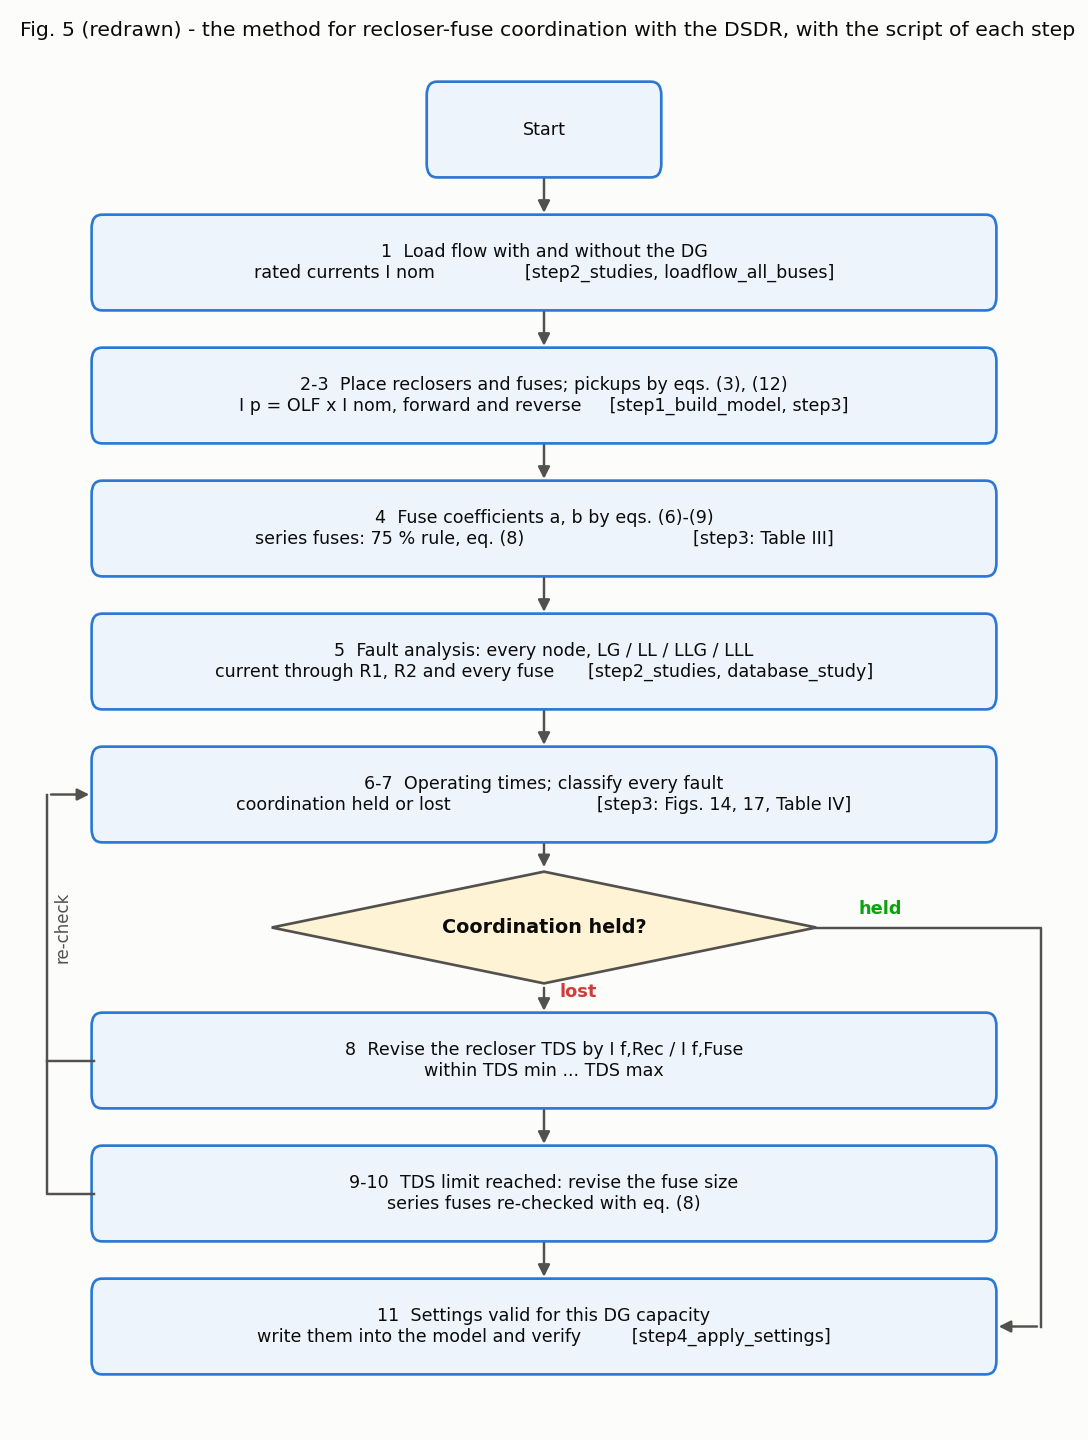
\includegraphics[width=0.78\textwidth]{flowchart.png}
\caption{Flowchart of the method as implemented (Fig.~5 of the reference paper).}
\label{fig:flow}
\end{figure}

\subsection{Model Setup in DIgSILENT \PF}
The earlier phase of the project used MATLAB/Simulink Specialized Power Systems. That model could not solve
the dynamic synchronous machine reliably, used a substitute relay curve, and left several fault cases
unresolved. The study was therefore rebuilt in DIgSILENT \PF{} 2021~SP2~\cite{pf2021}. The feeder is the
IEEE 13-node model of the DIgSILENT example library; its lines, loads and regulator taps were checked against
the IEEE data. The study case that includes the 115/4.16\,kV, 5\,MVA substation transformer is used, because
it reproduces the IEEE short-circuit benchmark~\cite{kersting2012}.

All studies are run through the \PF{} Python interface. Table~\ref{tab:scripts} lists the scripts; the
command \texttt{python run\_all.py} rebuilds the protection system and every result in about five minutes.

\begin{table}[H]
\centering\small
\begin{tabularx}{\textwidth}{@{}lL@{}}
\toprule
\hd\textbf{Script} & \textbf{Purpose} \\
\midrule
\texttt{step1\_build\_model.py} & Places the 15 fuses and the two reclosers, sets the DG to Table~I (\PF) \\
\texttt{step2\_studies.py} & Load flows and 273 short circuits; currents through every device (\PF) \\
\texttt{step3\_design\_and\_evaluate.py} & Settings by the paper's method, classification, Tables II--IV, TCC figures \\
\texttt{step4\_apply\_settings.py} & Writes the settings into \PF{} and compares \PF's trip times with step~3 \\
\texttt{step5\_fig10\_emt.py} & EMT simulation of the reclosing sequence (\PF) \\
\texttt{loadflow\_all\_buses.py}, \texttt{database\_study.py} & Load-flow and short-circuit database, DG out and in \\
\texttt{make\_coordination\_diagrams.py} & Single setting against dual setting on selected faults \\
\bottomrule
\end{tabularx}
\caption{Scripts of the study.}
\label{tab:scripts}
\end{table}

\subsection{Load Flow Analysis}
The load flow is the unbalanced three-phase AC load flow of \PF. It gives the rated current of every
protected branch (largest phase), the bus voltages per phase, and the current and its direction at the two
reclosers with and without the DG.

\subsection{Recloser Pickup Current}
The paper specifies an overload factor of 1.25. The pickup is 1.25 times the rated current of the protected
branch, eq.~\eqref{eq:ipfw}, and is then set on the nearest available tap of the relay.

\subsection{Short-Circuit Analysis}
Short circuits are calculated with the \emph{complete method} of \PF, which starts from the pre-fault load
flow. LG, LL, LLG and LLL faults are applied at every node for every phase combination that exists there,
with the DG out and in. The maximum fault current of a branch is a bolted fault at its nearest node; the
minimum is an LG fault through 3\ohm{} at its farthest node, as in the paper. The current through R1, R2,
every fuse and every branch of Table~II is stored for each fault.

\subsection{Mathematical Formulation of the DSDR}
The equations below are those of the reference paper; the numbering follows the paper.

\subsubsection{Forward Fast and Delayed Operating Time}
\begin{equation}
t^{fw}_{k,l,F} = TDS^{fw}_{k,F}\left[\frac{A^{fw}_{k}}{\left(I_{f,l}/I^{fw}_{p,k}\right)^{n^{fw}_{k}}-1}+B^{fw}_{k}\right]
\label{eq:tf}
\end{equation}
\begin{equation}
t^{fw}_{k,l,D} = TDS^{fw}_{k,D}\left[\frac{A^{fw}_{k}}{\left(I_{f,l}/I^{fw}_{p,k}\right)^{n^{fw}_{k}}-1}+B^{fw}_{k}\right]
\label{eq:td}
\end{equation}
The fast and the delayed operation of recloser $k$ for a fault at location $l$ use the same curve with two
time dials. $I_{f,l}$ is the fault current through the recloser and $I_p$ its pickup.

\subsubsection{Forward Pickup Current and Constraints}
\begin{equation}
I^{fw}_{p,k} = OLF \times I^{fw}_{nom,k}
\label{eq:ipfw}
\end{equation}
\begin{equation}
TDS_{k,min} < TDS^{fw}_{k,F},\; TDS^{fw}_{k,D} < TDS_{k,max}
\label{eq:tdslim}
\end{equation}
\begin{equation}
I_{p,k,min} < I^{fw}_{p,k} < I_{p,k,max}
\label{eq:iplim}
\end{equation}
The pickup lies above the load current and below the minimum fault current of the zone; the dials must stay
inside the range of the device.

\subsubsection{Fuse Characteristic and Coefficient}
\begin{equation}
\log t_{fuse,i} = a_i \log I_{f,i} + b_i
\label{eq:fuse}
\end{equation}
\begin{equation}
b_i = \log\!\left[\frac{t^{fw}_{k,F}+t^{fw}_{k,D}}{2}\right] - a_i \log I_{f,i}
\label{eq:bi}
\end{equation}
with $a_i=-1.8$. Equation~\eqref{eq:bi} places a single fuse midway between the fast and the delayed time at
the calibration current.

\subsubsection{Series Fuses}
\begin{equation}
t_{TCT,\,i} \le 0.75\; t_{MMT,\,i+1}
\label{eq:75}
\end{equation}
\begin{equation}
b_i = \log\!\left[t^{fw}_{k,F}+\frac{i\left(t^{fw}_{k,D}-t^{fw}_{k,F}\right)}{z+1}\right] - a_i \log I_{f,i}
\label{eq:biseries}
\end{equation}
where $z$ is the number of series fuses in the fault path and $i=1$ is the fuse closest to the fault.
Equation~\eqref{eq:biseries} divides the window between the two recloser times among the series fuses.

\subsubsection{Reverse Operating Times, Pickup and Constraints}
\begin{equation}
t^{rv}_{k,m,F} = TDS^{rv}_{k,F}\left[\frac{A^{rv}_{k}}{\left(I_{f,m}/I^{rv}_{p,k}\right)^{n^{rv}_{k}}-1}+B^{rv}_{k}\right]
\label{eq:trf}
\end{equation}
\begin{equation}
t^{rv}_{k,m,D} = TDS^{rv}_{k,D}\left[\frac{A^{rv}_{k}}{\left(I_{f,m}/I^{rv}_{p,k}\right)^{n^{rv}_{k}}-1}+B^{rv}_{k}\right]
\label{eq:trd}
\end{equation}
\begin{equation}
I^{rv}_{p,k} = OLF \times I^{rv}_{nom,k}
\label{eq:iprv}
\end{equation}
\begin{equation}
TDS_{k,min} < TDS^{rv}_{k,F},\; TDS^{rv}_{k,D} < TDS_{k,max}
\end{equation}
\begin{equation}
I_{p,k,min} < I^{rv}_{p,k} < I_{p,k,max}
\end{equation}
Here $m$ is a fault location upstream of the recloser. The reverse current is the contribution of the DG, and
the reverse pickup is based on the reverse load current that flows when the DG exports towards the
substation.

\subsection{Device Characteristics Used in the Model}
\label{sec:curves}
The paper names the devices but does not print their curve constants. The model uses the curves of the \PF{}
library for these devices.

\subsubsection{R1: GE IAC77B801A}
The extremely inverse IAC curve is
\begin{equation}
t = TDS\left[0.004+\frac{0.6379}{M-0.62}+\frac{1.7872}{(M-0.62)^2}+\frac{0.2461}{(M-0.62)^3}\right],
\qquad M=\frac{I_f}{I_p},
\label{eq:iac}
\end{equation}
valid from $M=1.5$ to $M=40$. This equation, and not eq.~\eqref{eq:tf} with standard IEEE constants,
reproduces the only worked example of the paper: for 4219\,A it gives 0.096\,s and 1.926\,s against the
paper's 0.097\,s and 1.932\,s.

\subsubsection{R2: GE/Alstom CDG34}
The CDG extremely inverse characteristic is a manufacturer's table of time against $M=I_f/I_s$ for time
multipliers from 0.1 to 1.0. It starts at twice the plug setting and is interpolated on log-log axes:
\begin{equation}
t = t_1\left(\frac{t_2}{t_1}\right)^{f},\qquad f=\frac{\ln(M/M_1)}{\ln(M_2/M_1)} .
\label{eq:cdg}
\end{equation}
The table is not defined below a multiplier of 0.1, so 0.1 is the fastest setting of this relay.

\subsubsection{Fuses}
The fuses are Gould-Shawmut A055C (5.5\,kV, E-rated) with their minimum-melting and total-clearing curves.
The fuse times are read from these curves at the current through the fuse with the same interpolation as
eq.~\eqref{eq:cdg}. The straight line of eq.~\eqref{eq:fuse} is used only to compute the coefficients of
Table~III; it was found that the paper's own figures also use A055C curves and not eq.~\eqref{eq:fuse}.

\subsection{Coordination Criteria}
A fault cell is classified as \emph{coordination exists} when all of the following hold:
\begin{equation}
t_{MMT}(I_{fuse}) > t_F \quad\text{for every recloser that feeds the fault through the fuse,}
\label{eq:crit1}
\end{equation}
\begin{equation}
t_{TCT}(I_{fuse}) < t_D \quad\text{for the same reclosers,}
\label{eq:crit2}
\end{equation}
together with the 75\,\% rule of eq.~\eqref{eq:75} for series fuses and a margin of at least 10~cycles
between the delayed curves of R2 and R1. A cell (node and fault type) is held only if every phase
combination of that fault type is held. The fuse and each recloser are evaluated at their own currents,
because with DG they differ.

\subsection{Design Procedure}
The steps of Figure~\ref{fig:flow} are applied as follows.
\begin{enumerate}
\item Load flow without DG: rated currents (Table~II) and pickups, eq.~\eqref{eq:ipfw}.
\item Short-circuit study: minimum and maximum fault currents (Table~II).
\item Recloser dials: R1 as given in the paper; R2 fast at the lowest dial, R2 delayed at the highest dial that
      stays 10~cycles below R1.
\item Fuse coefficients, eqs.~\eqref{eq:bi} and \eqref{eq:biseries} (Table~III), and check of the installed fuses.
\item Classification without DG; fuse revision until every cell is held.
\item DG connected, settings unchanged: classification (Fig.~14).
\item Reverse pickup of R2, eq.~\eqref{eq:iprv}, and reverse dials.
\item Revision of the dials (step~8 of the paper) and of the fuse sizes (step~9) until the cells are held.
\item Classification with the DSDR (Fig.~17) and operating times (Table~IV).
\item Verification: \PF's own relay and fuse models, and the EMT simulation.
\end{enumerate}

% =====================================================================================================
\chapterhead{FOUR}{SYSTEM MODELING AND SIMULATION SETUP}

\subsection{DIgSILENT \PF{} Environment}
The model is the project \emph{IEEE13 Yousaf2022 Replication} in \PF{} 2021~SP2. Load flows use the
unbalanced AC method, short circuits the complete method, and the time-domain study the EMT simulation with a
step of 0.1\,ms. The studies are run from Python~3.9 in engine mode; the same sequence can be started inside
\PF{} from one script object, which prints the report in the output window.

\subsection{IEEE 13-Node Feeder Model}
Figure~\ref{fig:sld} shows the feeder with the protection devices of the reference paper. The feeder has the
voltage regulator at the substation, overhead and cable sections, the 4.16/0.48\,kV transformer XFM-1, spot
and distributed loads, and two capacitors. The middle part of the distributed load on line 632--671 is placed
behind a short lateral (node DL) so that a fault there lies below its fuse, as drawn in the paper.

\begin{figure}[H]
\centering
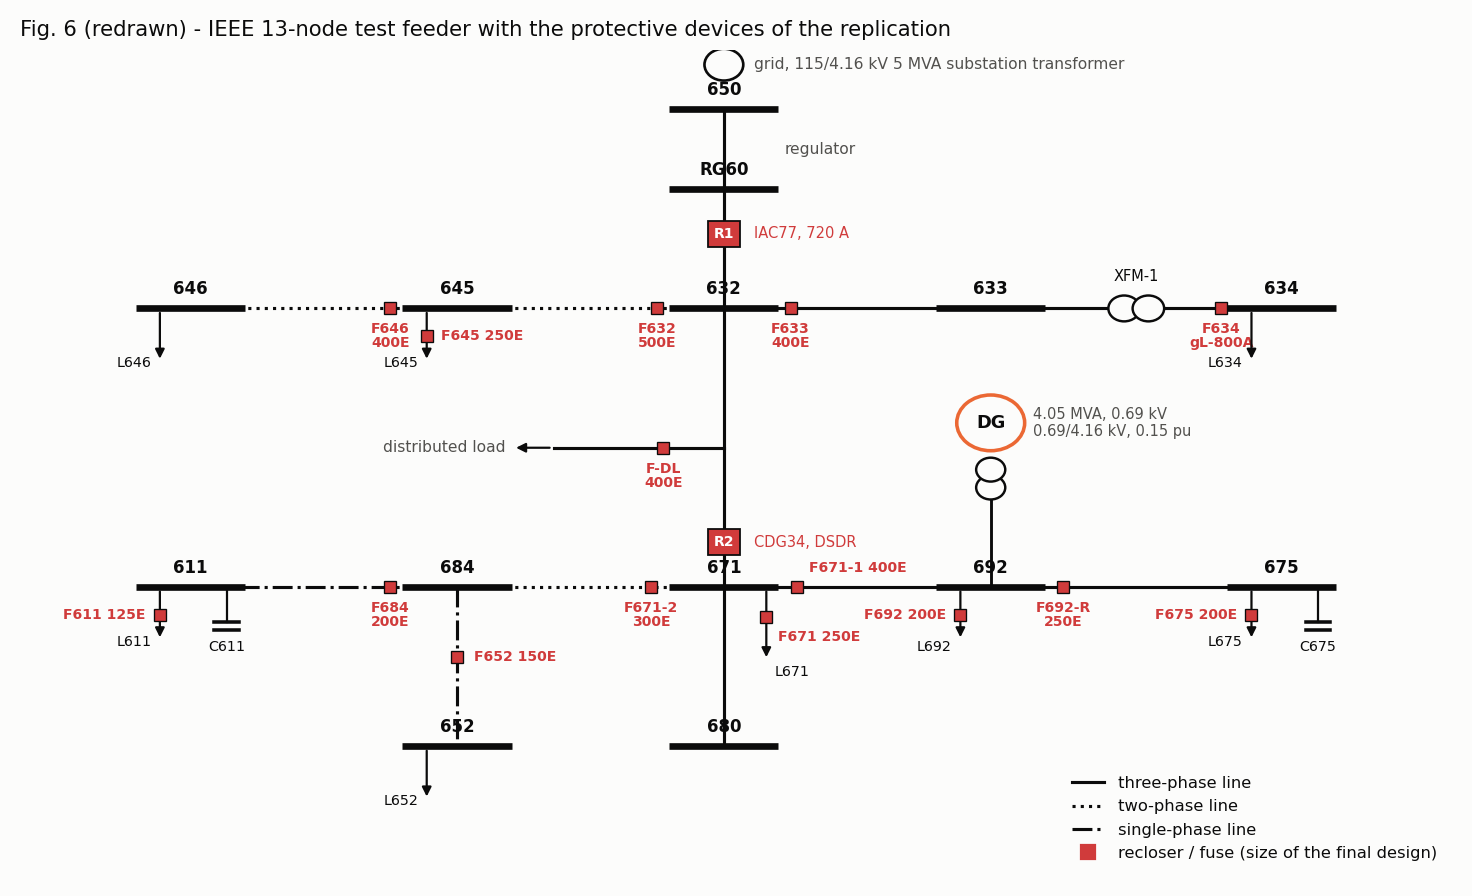
\includegraphics[width=\textwidth]{sld.png}
\caption{IEEE 13-node feeder with the reclosers R1 and R2, the fuses and the DG at node 692.}
\label{fig:sld}
\end{figure}

\subsection{Source and Feeder}
The source is an external grid at 115\,kV behind the 5\,MVA, 115/4.16\,kV substation transformer
($u_k = 8.06\,\%$). With this source the fault currents agree with the IEEE benchmark~\cite{kersting2012}
within about 2\,\% at every node. The alternative study case with a stiff 4.16\,kV source overstates the
fault levels by 20 to 65\,\% and is not used. The regulator taps are fixed at +10, +8 and +11.

\subsection{Distributed Generation Model}
The DG is a 4.05\,MVA, 0.69\,kV synchronous machine connected to node 692 through a 0.69/4.16\,kV
transformer with a leakage reactance of 0.15\,p.u. It is modelled with the standard synchronous-machine
model of \PF, round rotor, and the full data of Table~I of the paper. Table~\ref{tab:dg} compares the
paper's values with the values read back from the model. In the load flow the machine delivers 3.24\,MW and
controls its terminal voltage to 1.0\,p.u.; the paper does not give the operating point.

\begin{table}[H]
\centering\small
\begin{tabular}{@{}lcccc@{}}
\toprule
\hd\textbf{Parameter} & \textbf{Symbol} & \textbf{Paper} & \textbf{Model} & \textbf{Unit} \\
\midrule
Leakage reactance & $X_l$ & 0.05 & 0.05 & pu \\
Stator resistance & $R_a$ & 0.0014 & 0.0014 & pu \\
d-axis synchronous reactance & $X_d$ & 1.4 & 1.4 & pu \\
d-axis transient reactance & $X'_d$ & 0.231 & 0.231 & pu \\
d-axis subtransient reactance & $X''_d$ & 0.118 & 0.118 & pu \\
d-axis transient open-circuit time constant & $T'_{d0}$ & 5.5 & 5.5 & s \\
d-axis subtransient open-circuit time constant & $T''_{d0}$ & 0.05 & 0.05 & s \\
q-axis synchronous reactance & $X_q$ & 1.372 & 1.372 & pu \\
q-axis transient reactance & $X'_q$ & 0.8 & 0.8 & pu \\
q-axis subtransient reactance & $X''_q$ & 0.118 & 0.118 & pu \\
q-axis transient open-circuit time constant & $T'_{q0}$ & 1.25 & 1.25 & s \\
q-axis subtransient open-circuit time constant & $T''_{q0}$ & 0.19 & 0.19 & s \\
Mechanical starting time & $M = 2H$ & 1.5 & 1.5 & s \\
DG rating & $S_n$ & 4.05 & 4.05 & MVA \\
DG voltage & $U_n$ & 0.69 & 0.69 & kV \\
Step-up transformer, HV side & $U_{HV}$ & 4.16 & 4.16 & kV \\
Step-up transformer leakage reactance & $x_T$ & 0.15 & 0.15 & pu \\
\bottomrule
\end{tabular}
\caption{Parameters of the synchronous DG: reference paper against the \PF{} model.}
\label{tab:dg}
\end{table}

\subsection{Recloser Model}
R1 is at the feeder head (RG60--632). R2 is on line 632--671 at the 671 end; it is the DSDR, because with the
DG at 692 it carries forward current for faults at 671 and beyond and reverse current for faults towards 632.
Table~\ref{tab:settings} gives the settings. The forward and the reverse group of R2 are four relay units of
the CDG34 library type on two current transformers.

\begin{table}[H]
\centering\small
\begin{tabularx}{\textwidth}{@{}lLlll@{}}
\toprule
\hd\textbf{Recloser} & \textbf{Relay, CT} & \textbf{$1.25\,I_{nom}$} & \textbf{Setting} & \textbf{Dial fast / delayed} \\
\midrule
R1 forward & GE IAC77B801A, 900/5 & 734.6\,A & tap 4\,A = 720\,A & TDS 0.5 / 10 \\
R2 forward & CDG34, 1000/5 & 587.5\,A & plug 300\,A / 600\,A & TMS 0.1 / 1.0 \\
R2 reverse & CDG34, 500/5 & 315.3\,A & plug 150\,A / 300\,A & TMS 0.1 / 1.0 \\
\bottomrule
\end{tabularx}
\caption{Recloser settings. For R2 the fast plug is half and the delayed plug equal to $1.25\,I_{nom}$, because
the CDG curve starts at twice the plug setting.}
\label{tab:settings}
\end{table}

\subsection{Fuse Model}
Table~\ref{tab:fuses} lists the fifteen fuses. The starting size is the size drawn in the figures of the
reference paper where a figure shows the fuse (the fuse bands were digitised and matched to the A055C
library curves within 2\,\%), otherwise the size of the benchmark scheme~\cite{yousaf2020}. The last two
columns are the sizes after the fuse revision of the method without DG and with the DSDR.

\begin{table}[H]
\centering\footnotesize
\begin{tabularx}{\textwidth}{@{}llcccL@{}}
\toprule
\hd\textbf{Fuse} & \textbf{Location} & \textbf{Start} & \textbf{No DG} & \textbf{DSDR} & \textbf{Source of the starting size} \\
\midrule
F632 & lateral 632--645, at 632 & 400E & 400E & \textbf{500E} & Paper, Figs. 12, 15, 16 \\
F633 & lateral 632--633, at 632 & 250E & 250E & \textbf{400E} & Benchmark scheme~\cite{yousaf2020}, Table V \\
F634 & XFM-1, 0.48 kV side & gL-800A & gL-800A & gL-800A & Benchmark scheme~\cite{yousaf2020}, Table V \\
F645 & load at 645 & 250E & 250E & 250E & Benchmark scheme~\cite{yousaf2020}, Table V \\
F646 & line 645--646, at 645 & 300E & 300E & \textbf{400E} & Paper, Figs. 11, 15, 16 \\
F-DL & distributed-load lateral on 632--671 & 250E & 250E & \textbf{400E} & Benchmark scheme~\cite{yousaf2020}, Table V \\
F671 & load at 671 & 250E & 250E & 250E & Benchmark scheme~\cite{yousaf2020}, Table V \\
F671-1 & 671--692 (switch), at 671 & 300E & 300E & \textbf{400E} & Paper, Fig. 9 \\
F692 & load at 692 & 200E & 200E & 200E & Benchmark scheme~\cite{yousaf2020}, Table V \\
F692-R & cable 692--675, at 692 & 250E & 200E & \textbf{250E} & Paper, Fig. 9 \\
F675 & load at 675 & 200E & 200E & 200E & Benchmark scheme~\cite{yousaf2020}, Table V \\
F671-2 & lateral 671--684, at 671 & 300E & 300E & 300E & Paper, Fig. 8 \\
F684 & line 684--611, at 684 & 200E & 200E & 200E & Paper, Fig. 8 \\
F611 & load at 611 & 125E & 125E & 125E & Benchmark scheme~\cite{yousaf2020}, Table V \\
F652 & cable 684--652, at 684 & 150E & 150E & 150E & Benchmark scheme~\cite{yousaf2020}, Table V \\
\bottomrule
\end{tabularx}
\caption{Fuses and their sizes (A055C, E-rated). Bold: changed by the fuse revision with the DG.}
\label{tab:fuses}
\end{table}

\subsection{Fault Model}
Faults are applied at the nodes 632, 633, 634, 645, 646, DL, 671, 692, 675, 680, 684, 611 and 652. Only the
fault types that the phases of a node allow are applied, for example LL and LLG on phases b--c at 645 and
646, and LG only at 611 and 652. This gives 39 node/fault-type cells. The faults of the paper's
figures are added with their fault impedances.

\subsection{Measurement and Data Acquisition}
\label{sec:assumptions}
For every fault the phase currents through R1, R2 and each fuse are read from the short-circuit result. The
operating current of a device is its largest phase current. The forward direction is away from the grid; R2
sits at the 671 end of its line, where \PF{} counts the current positive into the line, so its values are
multiplied by $-1$. The following values are not given in the paper and were chosen:
\begin{itemize}
\item the source (IEEE benchmark substation transformer) and the complete short-circuit method;
\item the tap and the current transformer of R1 (720\,A reproduces the paper's worked example);
\item all settings of R2 (Table~\ref{tab:settings}), derived from eqs.~\eqref{eq:ipfw} and \eqref{eq:iprv}
      and from the curve starts visible in the paper's figures;
\item the fault behind each row of Table~IV: bolted LLL, LL at two-phase nodes, LG at single-phase nodes;
\item the reclosing dead time (0.2\,s, read from the paper's Fig.~10) and a breaker time of three cycles in
      the EMT study.
\end{itemize}

\subsection{Simulation Cases}
\begin{table}[H]
\centering\small
\begin{tabularx}{\textwidth}{@{}llLL@{}}
\toprule
\hd\textbf{Case} & \textbf{DG} & \textbf{Faults} & \textbf{Purpose} \\
\midrule
Load flow & out / in & -- & Rated currents, voltages, direction at R1 and R2 \\
Maximum faults & out / in & All nodes, LG/LL/LLG/LLL, all phase combinations, bolted & Classification, Tables II--IV \\
Minimum faults & out / in & LG through 3\ohm{} at all nodes & $I_{f,min}$, pickup check \\
Figure faults & in & The faults of Figs.~8--13, 15, 16 of the paper & TCC comparison \\
EMT & out / in & LL a--c at 684 through 0.2\ohm & Reclosing sequence (Fig.~10) \\
\bottomrule
\end{tabularx}
\caption{Simulation cases.}
\label{tab:cases}
\end{table}

% =====================================================================================================
\chapterhead{FIVE}{RESULTS OBTAINED}

\subsection{Load-Flow Results}
Table~\ref{tab:volt} gives the bus voltages with and without the DG. Without DG the lowest voltage is
0.971\,p.u. (phase c at 611). The DG raises the voltages of the loaded phases a and c at node 671 and beyond
by about 0.03 to 0.05\,p.u.

\begin{table}[H]
\centering\small
\begin{tabular}{@{}lcccccc@{}}
\toprule
\hd & \multicolumn{3}{c}{\textbf{Without DG (p.u.)}} & \multicolumn{3}{c}{\textbf{With DG (p.u.)}} \\
\hd\textbf{Bus} & \textbf{A} & \textbf{B} & \textbf{C} & \textbf{A} & \textbf{B} & \textbf{C} \\
\midrule
650 & 0.9981 & 1.0170 & 0.9979 & 1.0084 & 1.0200 & 1.0057 \\
RG60 & 1.0605 & 1.0679 & 1.0665 & 1.0715 & 1.0710 & 1.0748 \\
632 & 1.0187 & 1.0616 & 1.0142 & 1.0482 & 1.0640 & 1.0361 \\
633 & 1.0158 & 1.0588 & 1.0124 & 1.0454 & 1.0611 & 1.0344 \\
634 & 0.9918 & 1.0406 & 0.9936 & 1.0221 & 1.0430 & 1.0161 \\
645 & -- & 1.0540 & 1.0106 & -- & 1.0563 & 1.0325 \\
646 & -- & 1.0522 & 1.0085 & -- & 1.0546 & 1.0304 \\
DL & 1.0028 & 1.0666 & 0.9939 & 1.0407 & 1.0685 & 1.0221 \\
671 & 0.9877 & 1.0722 & 0.9753 & 1.0334 & 1.0738 & 1.0094 \\
692 & 0.9877 & 1.0722 & 0.9753 & 1.0334 & 1.0738 & 1.0094 \\
675 & 0.9809 & 1.0767 & 0.9729 & 1.0271 & 1.0781 & 1.0072 \\
680 & 0.9877 & 1.0722 & 0.9753 & 1.0334 & 1.0738 & 1.0094 \\
684 & 0.9859 & -- & 0.9732 & 1.0315 & -- & 1.0074 \\
652 & 0.9811 & -- & -- & 1.0265 & -- & -- \\
611 & -- & -- & 0.9712 & -- & -- & 1.0055 \\
\bottomrule
\end{tabular}
\caption{Bus voltages from the unbalanced load flow, without and with the DG.}
\label{tab:volt}
\end{table}

Table~\ref{tab:lf} shows the load current at the two reclosers. With the DG the current through R2 reverses:
252.2\,A flows from 671 towards 632. This reverse load current is the basis of the reverse pickup,
eq.~\eqref{eq:iprv}.

\begin{table}[H]
\centering\small
\begin{tabular}{@{}lcccc@{}}
\toprule
\hd\textbf{Device} & \textbf{Without DG (A)} & \textbf{Direction} & \textbf{With DG (A)} & \textbf{Direction} \\
\midrule
R1 & $+587.7$ & forward & $+284.9$ & forward \\
R2 & $+470.0$ & forward & $-252.2$ & reverse \\
\bottomrule
\end{tabular}
\caption{Load current at the reclosers (largest phase; + is forward, away from the grid).}
\label{tab:lf}
\end{table}

\subsection{Branch Currents and Fault Levels (Table II)}
Table~\ref{tab:t2} reproduces Table~II of the paper. The rated currents agree within 2\,\% on every branch.
The minimum fault currents are of the same size as the paper's. The maximum fault currents are lower, by 4 to 60\,\% on the feeder branches: the
model follows the IEEE benchmark, while several of the paper's values exceed its own value at the feeder
head (5.41\,kA), which is not possible on a radial feeder without DG.

\begin{table}[H]
\centering\footnotesize
\begin{tabular}{@{}lcccccccc@{}}
\toprule
\hd & \multicolumn{3}{c}{\textbf{$I_{nom}$ (A)}} & \multicolumn{2}{c}{\textbf{$I_{f,min}$ (kA)}} & \multicolumn{3}{c}{\textbf{$I_{f,max}$ (kA)}} \\
\hd\textbf{Branch} & \textbf{model} & \textbf{paper} & \textbf{dev.\,\%} & \textbf{model} & \textbf{paper} & \textbf{model} & \textbf{paper} & \textbf{dev.\,\%} \\
\midrule
RG60--632 & 587.7 & 587.1 & $+0.1$ & 1.07 & 1.24 & 4.73 & 5.41 & $-13$ \\
632--633 & 81.0 & 81.1 & $-0.1$ & 0.76 & 0.72 & 4.1 & 6.73 & $-39$ \\
632--645 & 143.1 & 143.3 & $-0.1$ & 0.73 & 0.93 & 3.42 & 4.25 & $-20$ \\
632--671 & 470.0 & 478.2 & $-1.7$ & 0.88 & 1.08 & 3.39 & 4.52 & $-25$ \\
XFM1-HV side & 81.0 & 81.1 & $-0.1$ & 0.08 & 0.73 & 1.81 & 6.48 & $-72$ \\
XFM1-LV side & 706.4 & 704.7 & $+0.2$ & 0.71 & 0.59 & 15.67 & 18.76 & $-16$ \\
645--646 & 66.1 & 64.9 & $+1.8$ & 0.73 & 0.84 & 3.11 & 3.64 & $-15$ \\
671--692 & 229.7 & 229.3 & $+0.2$ & 0.74 & 0.78 & 3.39 & 3.69 & $-8$ \\
671--684 & 71.1 & 70.9 & $+0.3$ & 0.66 & 0.69 & 2.66 & 3.47 & $-23$ \\
671--680 & 0.0 & 0.0 & -- & 0.64 & 0.59 & 2.93 & 6.25 & $-53$ \\
692--675 & 205.9 & 205.9 & $+0.0$ & 0.74 & 0.71 & 3.15 & 7.83 & $-60$ \\
684--611 & 71.1 & 70.8 & $+0.4$ & 0.68 & 0.63 & 1.86 & 1.93 & $-4$ \\
684--652 & 63.0 & 63.1 & $-0.2$ & 0.66 & 0.66 & 1.87 & 2.67 & $-30$ \\
\bottomrule
\end{tabular}
\caption{Rated, minimum and maximum fault current of the protected branches without DG (Table~II of the paper).
XFM1 HV side: the model values are the 4.16\,kV currents for a fault on the 0.48\,kV side, so this row is not
comparable with the paper's.}
\label{tab:t2}
\end{table}

\subsection{Recloser Pickup Currents and Settings}
With the rated currents of Table~\ref{tab:t2}, eq.~\eqref{eq:ipfw} gives 734.6\,A for R1 and 587.5\,A for R2
forward. The settings actually applied are those of Table~\ref{tab:settings}. Without DG both pickups are
below the lowest minimum fault current of their zones (1074\,A and 879\,A).

\subsection{Short-Circuit Results With and Without DG}
Table~\ref{tab:fault} gives the largest fault current at each node and the current through the two reclosers.
The DG raises the fault current at every node, by 38\,\% at 632 and by 64\,\% at 671. For faults at 632,
633, 645, 646 and DL the current through R2 becomes negative: R2 then carries only the DG contribution, 1.1
to 2.0\,kA, in the reverse direction, while R1 still carries the grid contribution.

\begin{table}[H]
\centering\footnotesize
\begin{tabular}{@{}llcccccc@{}}
\toprule
\hd & & \multicolumn{2}{c}{\textbf{$I_{f,max}$ at the fault (A)}} & \multicolumn{2}{c}{\textbf{Through R1 (A)}} & \multicolumn{2}{c}{\textbf{Through R2 (A)}} \\
\hd\textbf{Bus} & \textbf{Fault} & \textbf{no DG} & \textbf{DG} & \textbf{no DG} & \textbf{DG} & \textbf{no DG} & \textbf{DG} \\
\midrule
632 & LLL ABC & 4735 & 6526 & $+4735$ & $+4734$ & $+0$ & $-1813$ \\
633 & LLL ABC & 4102 & 5426 & $+4162$ & $+3970$ & $+66$ & $-1500$ \\
634 & LLL ABC & 15671 & 17608 & $+2034$ & $+1611$ & $+298$ & $-618$ \\
645 & LLG BC & 3418 & 4341 & $+3528$ & $+3330$ & $+478$ & $-1262$ \\
646 & LLG BC & 3112 & 3854 & $+3192$ & $+3000$ & $+475$ & $-1135$ \\
671 & LLL ABC & 3390 & 5564 & $+3413$ & $+3412$ & $+3390$ & $+3391$ \\
692 & LLL ABC & 3390 & 5564 & $+3413$ & $+3412$ & $+3390$ & $+3391$ \\
675 & LLL ABC & 3151 & 5022 & $+3202$ & $+3090$ & $+3174$ & $+3050$ \\
680 & LLL ABC & 2930 & 4460 & $+3006$ & $+2789$ & $+2976$ & $+2757$ \\
684 & LLG AC & 2655 & 4107 & $+2836$ & $+2669$ & $+2744$ & $+2651$ \\
652 & LG A & 1874 & 2239 & $+2094$ & $+1795$ & $+2059$ & $+1761$ \\
611 & LG C & 1857 & 2236 & $+2084$ & $+1814$ & $+1991$ & $+1718$ \\
DL & LLL ABC & 3946 & 5902 & $+3959$ & $+3954$ & $+1$ & $-1972$ \\
\bottomrule
\end{tabular}
\caption{Maximum fault current and recloser currents without and with the DG (+ forward, $-$ reverse).}
\label{tab:fault}
\end{table}

\subsection{Fuse Coefficients (Table III)}
Table~\ref{tab:t3} gives the fuse coefficients of eq.~\eqref{eq:biseries}. With $i$ counted from the fault,
as the paper defines it, the values differ from the paper's Table~III. With $i$ counted from the source they
agree within 0.05 for the series fuses of R1's zone; in R2's zone the agreement is weaker (within 0.25),
because the settings of R2 are not published. The paper's table therefore applies the equation with the index
reversed, which would make the upstream fuse faster than the downstream one. The last two columns give the
installed fuse and its melting time at the same current; it is much shorter than the time the equation asks
for, because real fuse curves are steeper than the slope $-1.8$.

\begin{table}[H]
\centering\footnotesize
\begin{tabular}{@{}lcccccccccc@{}}
\toprule
\hd\textbf{Fuse} & \textbf{$I_f$ (A)} & \textbf{$i/z$} & \textbf{$t_F$ (s)} & \textbf{$t_D$ (s)} & \textbf{$t_{fuse}$ (s)} &
\textbf{$b_i$} & \textbf{$b_i$ rev.} & \textbf{paper} & \textbf{Size} & \textbf{$t_{MMT}$ (s)} \\
\midrule
F632 & 3418 & 2/2 & 0.133 & 2.670 & 1.824 & 6.62 & 6.35 & 6.38 & 400E & 0.512 \\
F633 & 4102 & 1/1 & 0.100 & 2.008 & 1.054 & 6.53 & 6.53 & 6.83 & 250E & 0.102 \\
F634 & 15671 & 1/2 & 0.439 & 8.772 & 3.217 & 8.06 & 8.33 & 8.32 & gL-800A & 0.021 \\
F645 & 3418 & 1/2 & 0.133 & 2.670 & 0.979 & 6.35 & 6.62 & 6.65 & 250E & 0.158 \\
F646 & 3112 & 1/2 & 0.156 & 3.115 & 1.142 & 6.35 & 6.62 & 6.67 & 300E & 0.273 \\
F-DL & 3946 & 1/1 & 0.106 & 2.130 & 1.118 & 6.52 & 6.52 & 6.54 & 250E & 0.112 \\
F671 & 3390 & 1/1 & 0.054 & 1.601 & 0.827 & 6.27 & 6.27 & 6.08 & 250E & 0.161 \\
F671-1 & 3390 & 3/3 & 0.054 & 1.601 & 1.214 & 6.44 & 6.00 & 5.85 & 300E & 0.218 \\
F692 & 3390 & 1/2 & 0.054 & 1.601 & 0.569 & 6.11 & 6.39 & 6.13 & 200E & 0.094 \\
F692-R & 3151 & 2/3 & 0.057 & 1.829 & 0.943 & 6.27 & 6.27 & 6.14 & 200E & 0.112 \\
F675 & 3151 & 1/3 & 0.057 & 1.829 & 0.500 & 6.00 & 6.44 & 6.19 & 200E & 0.112 \\
F671-2 & 2655 & 3/3 & 0.069 & 2.572 & 1.946 & 6.45 & 6.01 & 5.87 & 300E & 0.428 \\
F684 & 1857 & 2/3 & 0.113 & 5.778 & 2.946 & 6.35 & 6.35 & 6.15 & 200E & 0.465 \\
F611 & 1857 & 1/3 & 0.113 & 5.778 & 1.530 & 6.07 & 6.52 & 6.19 & 125E & 0.120 \\
F652 & 1874 & 1/2 & 0.112 & 5.660 & 1.961 & 6.18 & 6.47 & 6.17 & 150E & 0.207 \\
\bottomrule
\end{tabular}
\caption{Fuse coefficients, eq.~(9), $a_i=-1.8$ (Table~III of the paper). ``$b_i$ rev.'': index $i$ counted
from the source. Size and $t_{MMT}$: fuse of the design without DG at the same current.}
\label{tab:t3}
\end{table}

\subsection{Conventional Coordination Without DG}
With the starting fuse sizes 35 of the 39 cells are coordinated. The four lost cells are the faults
at 675, where the series pair F692-R (250E) and F671-1 (300E) breaks the 75\,\% rule. The fuse revision of
the method changes F692-R to 200E, after which all 39 cells are coordinated. Figures~\ref{fig:f8}
and \ref{fig:f9} show two of the paper's cases: R2's fast curve lies below the fuses and its delayed curve
above them.

\begin{figure}[H]
\centering
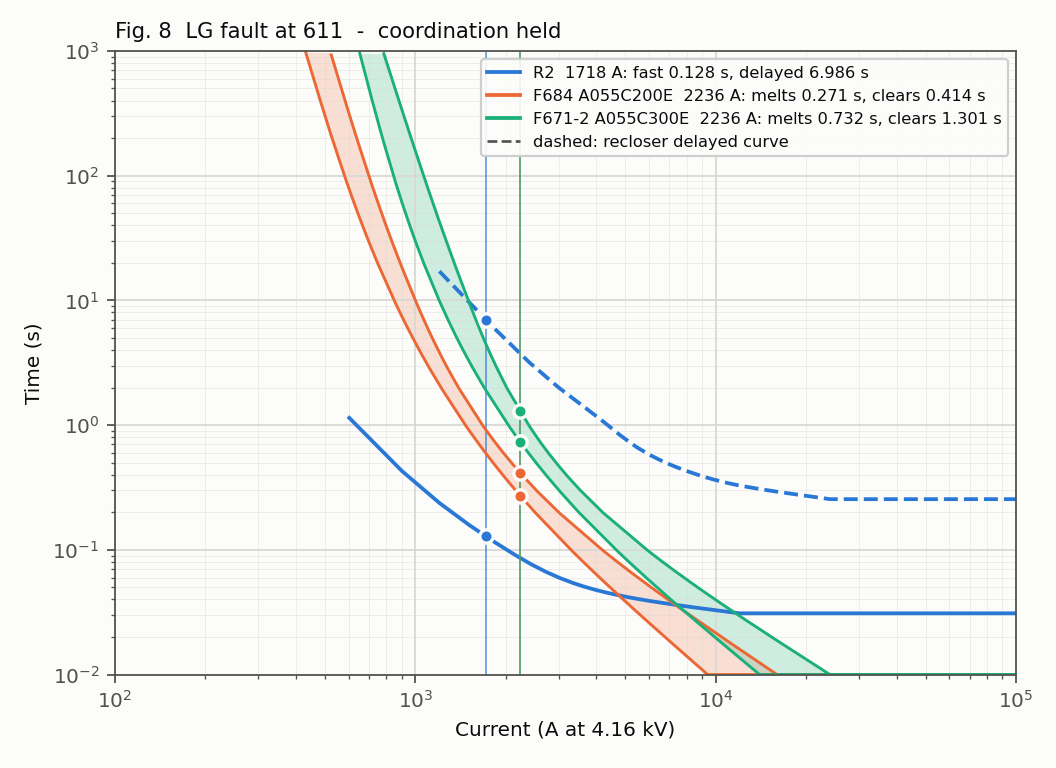
\includegraphics[width=0.68\textwidth]{fig08.png}
\caption{LG fault at 611 (Fig.~8 of the paper): R2 forward, fuses F684 and F671-2.}
\label{fig:f8}
\end{figure}

\begin{figure}[H]
\centering
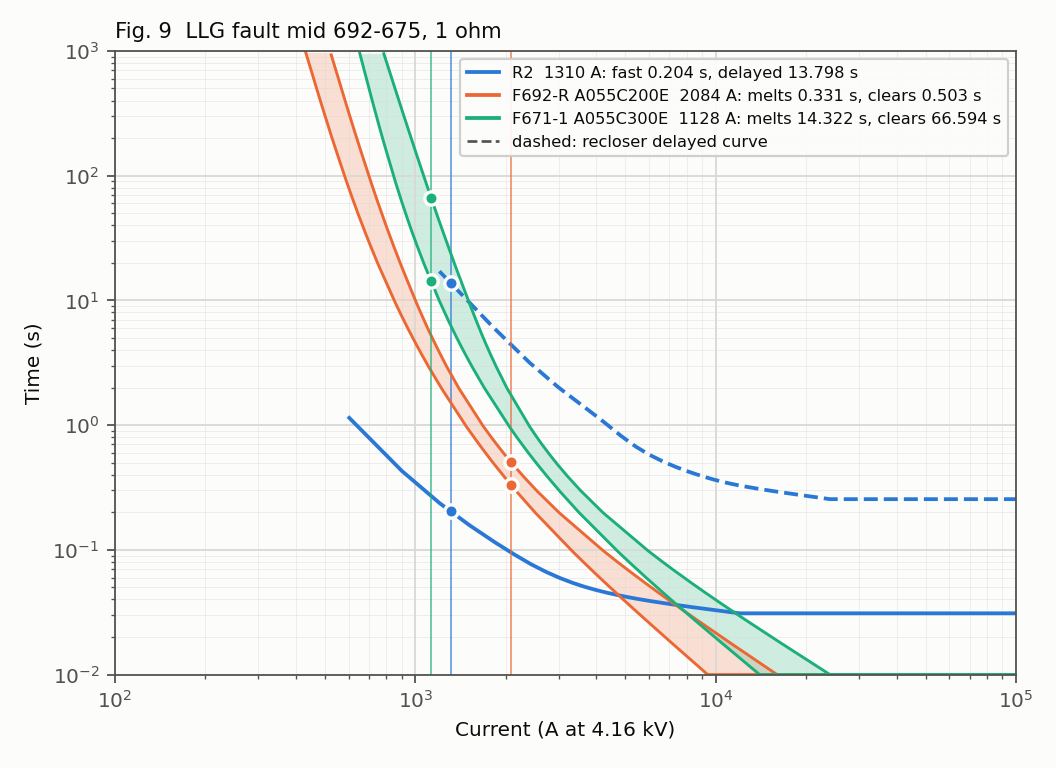
\includegraphics[width=0.68\textwidth]{fig09.png}
\caption{LLG fault at the middle of 692--675 through 1\ohm{} (Fig.~9 of the paper).}
\label{fig:f9}
\end{figure}

\subsection{Coordination With DG and a Conventional R2 (Fig. 14)}
With the DG connected and the settings unchanged, coordination is held in 24 of 39 cells
(Table~\ref{tab:g14}, Figure~\ref{fig:f14}). The lost cells are at 633, 645, 646, DL and 675: the fuse now
carries the grid and the DG current and melts before the fast trip, and for some LG faults the single-setting
R2 does not pick up the reverse DG current at all. 29 of the 39 cells have the same status
as in the paper's Fig.~14; the paper marks nine cells as lost, the model fifteen. The differences are mainly at
633 and DL, which are lost in the model and held in the paper because the model's fuses there have almost no
margin even without DG, and at 645, where the model holds two cells that the paper marks as lost.

\begin{table}[H]
\centering\footnotesize
\setlength{\tabcolsep}{4.5pt}
\begin{tabular}{@{}l*{12}{c}@{}}
\toprule
\hd\textbf{Fault} & 632 & 633 & 645 & 646 & DL & 671 & 692 & 675 & 680 & 684 & 611 & 652 \\
\midrule
LG (model) & \ok & \no & \no & \no & \no & \ok & \ok & \ok & \ok & \ok & \ok & \ok \\
LG (paper) & \ok & \ok & \no & \ok & \ok & \ok & \ok & \ok & \ok & \ok & \ok & \ok \\
LL (model) & \ok & \no & \ok & \no & \no & \ok & \ok & \no & \ok & \ok & -- & -- \\
LL (paper) & \ok & \ok & \no & \no & \ok & \ok & \ok & \ok & \ok & \ok & -- & -- \\
LLG (model) & \ok & \no & \ok & \no & \no & \ok & \ok & \no & \ok & \ok & -- & -- \\
LLG (paper) & \ok & \no & \no & \no & \ok & \ok & \ok & \no & \ok & \ok & -- & -- \\
LLL (model) & \ok & \no & -- & -- & \no & \ok & \ok & \no & \ok & -- & -- & -- \\
LLL (paper) & \ok & \no & -- & -- & \ok & \ok & \ok & \no & \ok & -- & -- & -- \\
\bottomrule
\end{tabular}
\caption{Coordination status with DG and a conventional R2 (Fig.~14 of the paper): model and paper.
$\checkmark$ exists, $\times$ does not exist, -- not applicable.}
\label{tab:g14}
\end{table}

\begin{figure}[H]
\centering
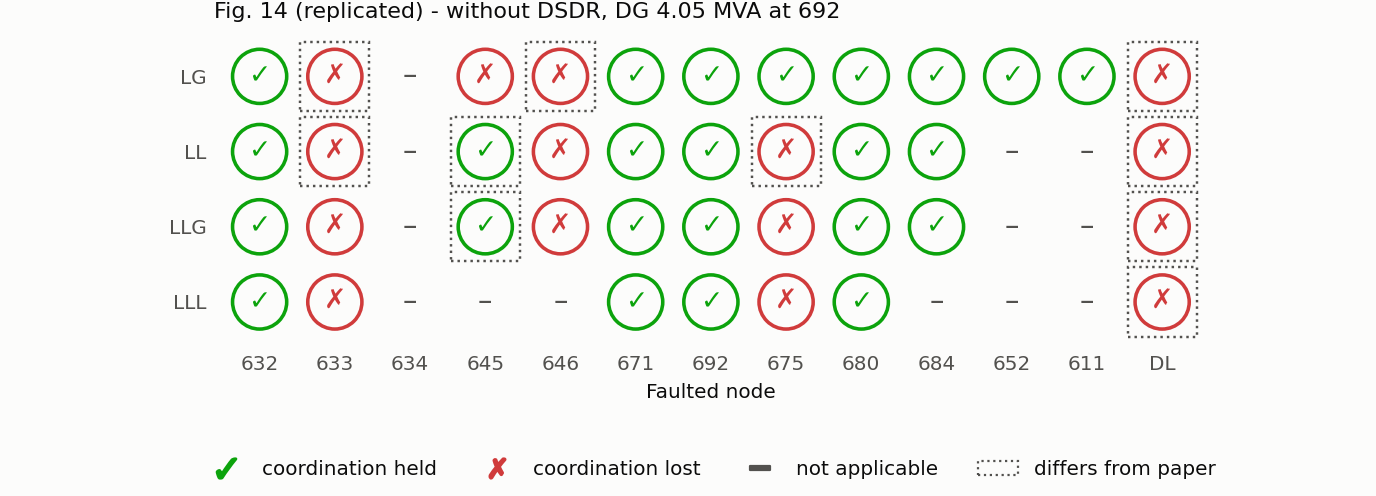
\includegraphics[width=0.9\textwidth]{fig14.png}
\caption{Coordination status with DG, without the DSDR (replication of Fig.~14).}
\label{fig:f14}
\end{figure}

Figures~\ref{fig:f11} to \ref{fig:f13} show the paper's three cases with the conventional R2.

\begin{figure}[H]
\centering
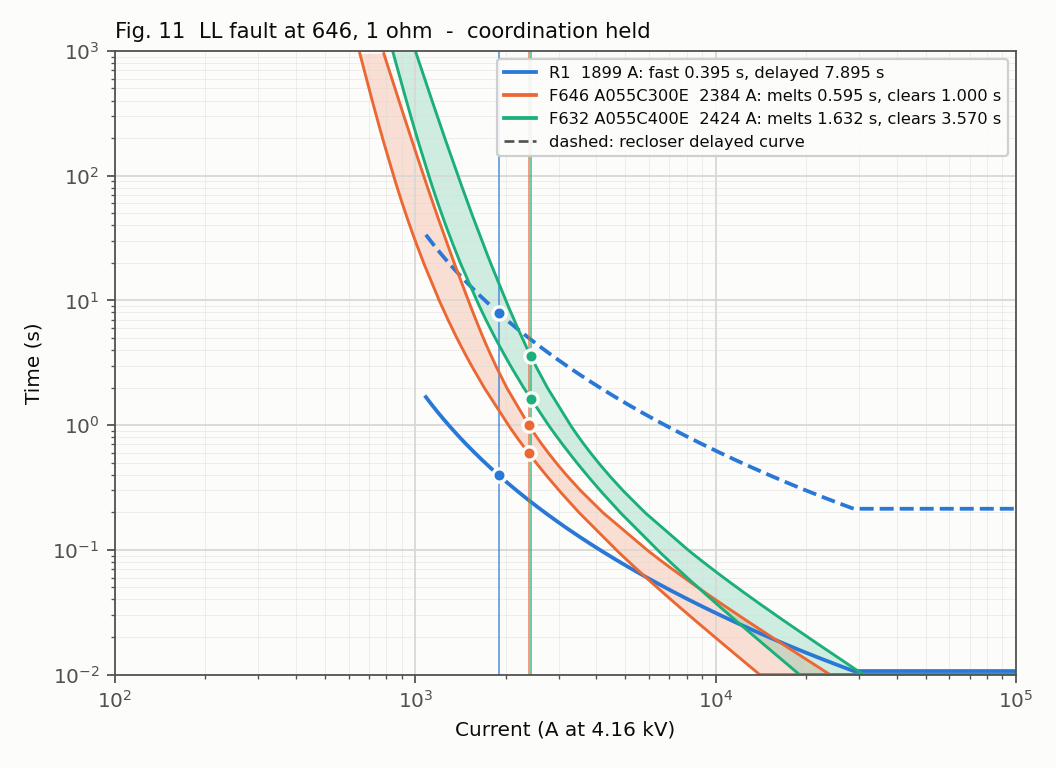
\includegraphics[width=0.68\textwidth]{fig11.png}
\caption{LL fault at 646 through 1\ohm: R1 with F646 and F632 (Fig.~11 of the paper).}
\label{fig:f11}
\end{figure}

\begin{figure}[H]
\centering
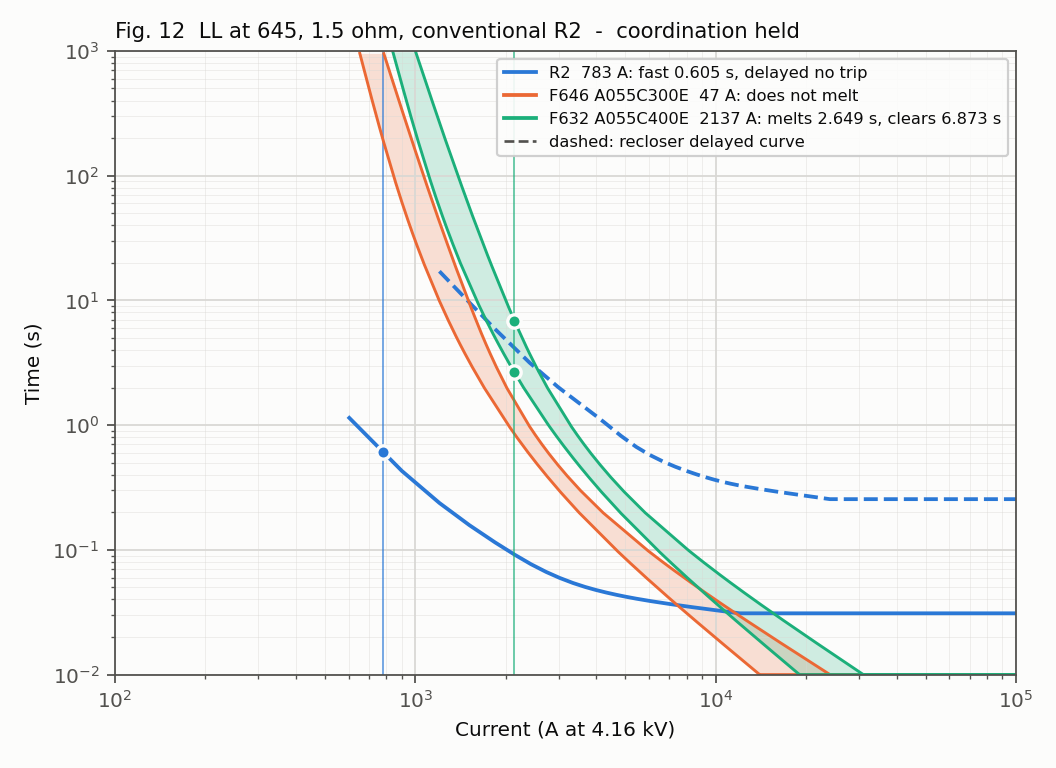
\includegraphics[width=0.68\textwidth]{fig12.png}
\caption{LL fault at 645 through 1.5\ohm, conventional R2 (Fig.~12 of the paper).}
\label{fig:f12}
\end{figure}

\begin{figure}[H]
\centering
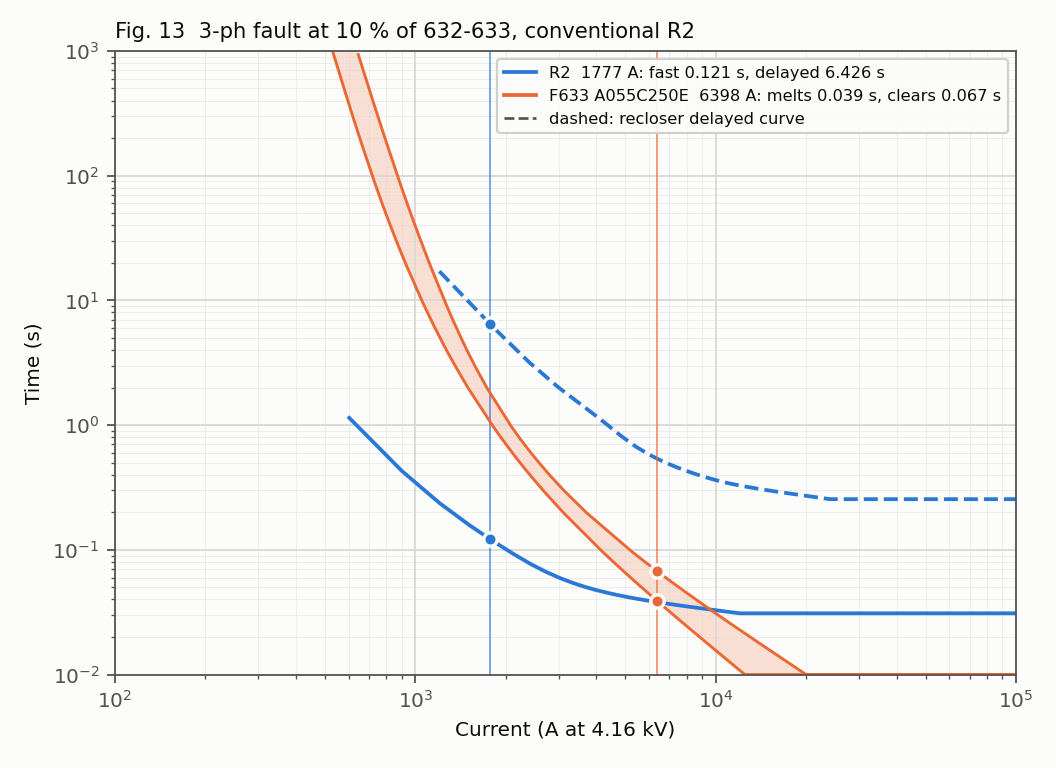
\includegraphics[width=0.68\textwidth]{fig13.png}
\caption{Three-phase fault at 10\,\% of line 632--633, conventional R2 (Fig.~13 of the paper).}
\label{fig:f13}
\end{figure}

\subsection{DSDR Settings and Fuse Revision}
The reverse load current of R2 is 252.2\,A, so eq.~\eqref{eq:iprv} gives a reverse pickup of 315.3\,A. The
reverse group is set on a 500/5 current transformer with plugs of 150\,A (fast) and 300\,A (delayed) and the
same time multipliers 0.1 and 1.0 (Figure~\ref{fig:f3}). Step~8 of the method (revising the dials) could not
improve any lost case, because R1 is already at both ends of the IAC dial range (0.5 and 10) and R2 at both
ends of the CDG table (0.1 and 1.0). Step~9 (revising the fuses) was therefore needed: F632 to 500E; F633,
F646, F-DL and F671-1 to 400E; F692-R to 250E (Table~\ref{tab:fuses}).

\begin{figure}[H]
\centering
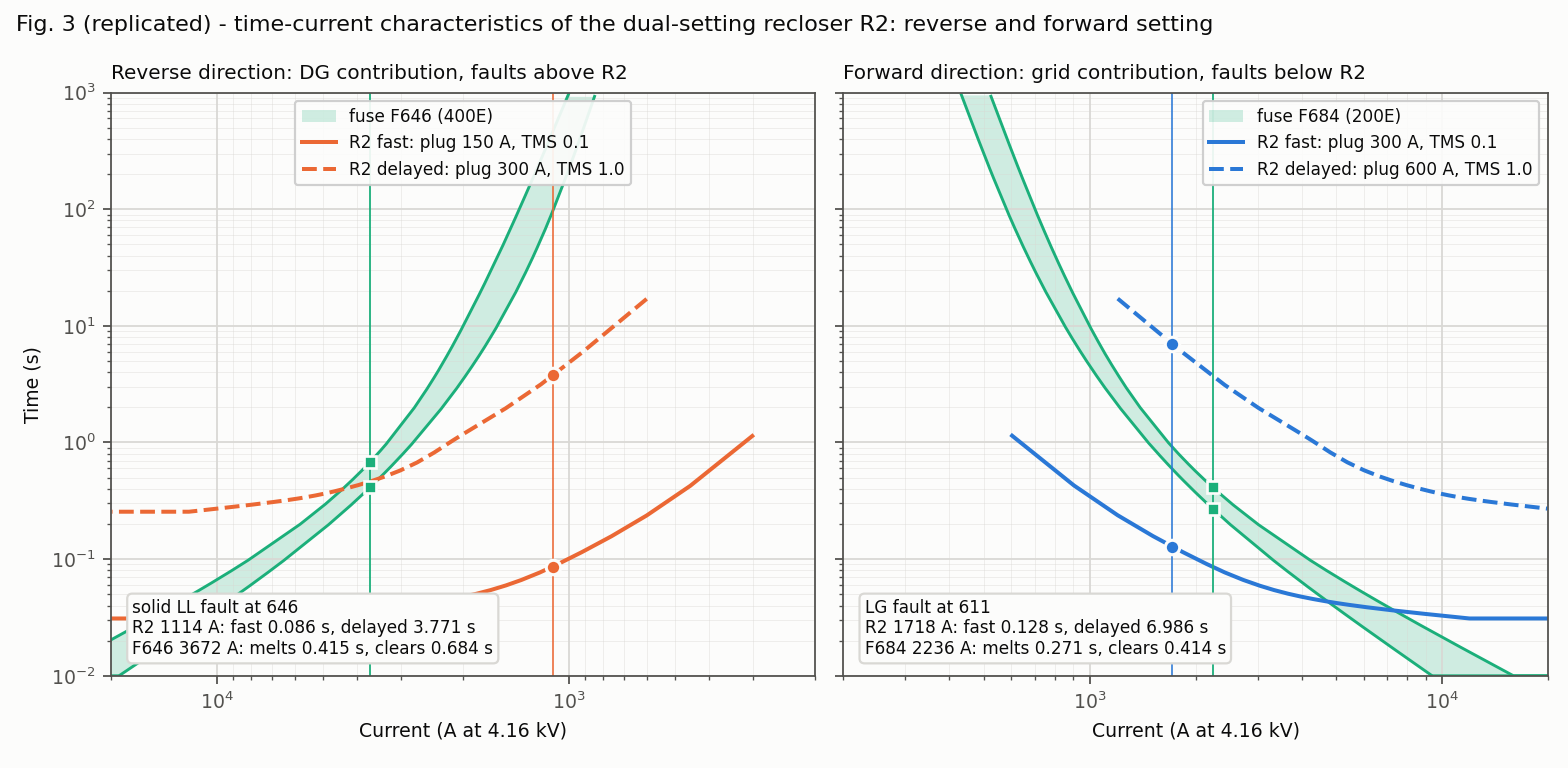
\includegraphics[width=\textwidth]{fig03.png}
\caption{The two setting groups of R2: reverse (DG contribution, faults towards 632) and forward (grid
contribution, faults beyond 671), each with one fault of the model.}
\label{fig:f3}
\end{figure}

\subsection{Coordination With the DSDR (Fig. 17)}
With R2 as a DSDR and the revised fuses, coordination is held in 38 of 39 cells
(Table~\ref{tab:g17}, Figure~\ref{fig:f17}). With the same fuses and a single-setting R2 only
31 cells are held. The dual setting itself therefore restores seven cells: all four fault types at
633, and the LG faults at 645, 646 and DL.

The cell that remains lost is the LG fault at 692. F671-1 must be 400E to stay selective with F692-R, but it
then clears after R2's delayed trip (7.6\,s against 4.0\,s), and R2's delayed dial is already at its maximum.

\begin{table}[H]
\centering\footnotesize
\setlength{\tabcolsep}{4.5pt}
\begin{tabular}{@{}l*{12}{c}@{}}
\toprule
\hd\textbf{Fault, R2} & 632 & 633 & 645 & 646 & DL & 671 & 692 & 675 & 680 & 684 & 611 & 652 \\
\midrule
LG, single setting & \ok & \no & \no & \no & \no & \ok & \no & \ok & \ok & \ok & \ok & \ok \\
LG, dual setting & \ok & \ok & \ok & \ok & \ok & \ok & \no & \ok & \ok & \ok & \ok & \ok \\
LL, single setting & \ok & \no & \ok & \ok & \ok & \ok & \ok & \ok & \ok & \ok & -- & -- \\
LL, dual setting & \ok & \ok & \ok & \ok & \ok & \ok & \ok & \ok & \ok & \ok & -- & -- \\
LLG, single setting & \ok & \no & \ok & \ok & \ok & \ok & \ok & \ok & \ok & \ok & -- & -- \\
LLG, dual setting & \ok & \ok & \ok & \ok & \ok & \ok & \ok & \ok & \ok & \ok & -- & -- \\
LLL, single setting & \ok & \no & -- & -- & \ok & \ok & \ok & \ok & \ok & -- & -- & -- \\
LLL, dual setting & \ok & \ok & -- & -- & \ok & \ok & \ok & \ok & \ok & -- & -- & -- \\
\bottomrule
\end{tabular}
\caption{Coordination status with DG and the revised fuses: single-setting R2 against dual-setting R2 (Fig.~17
of the paper, in which every cell exists).}
\label{tab:g17}
\end{table}

\begin{figure}[H]
\centering
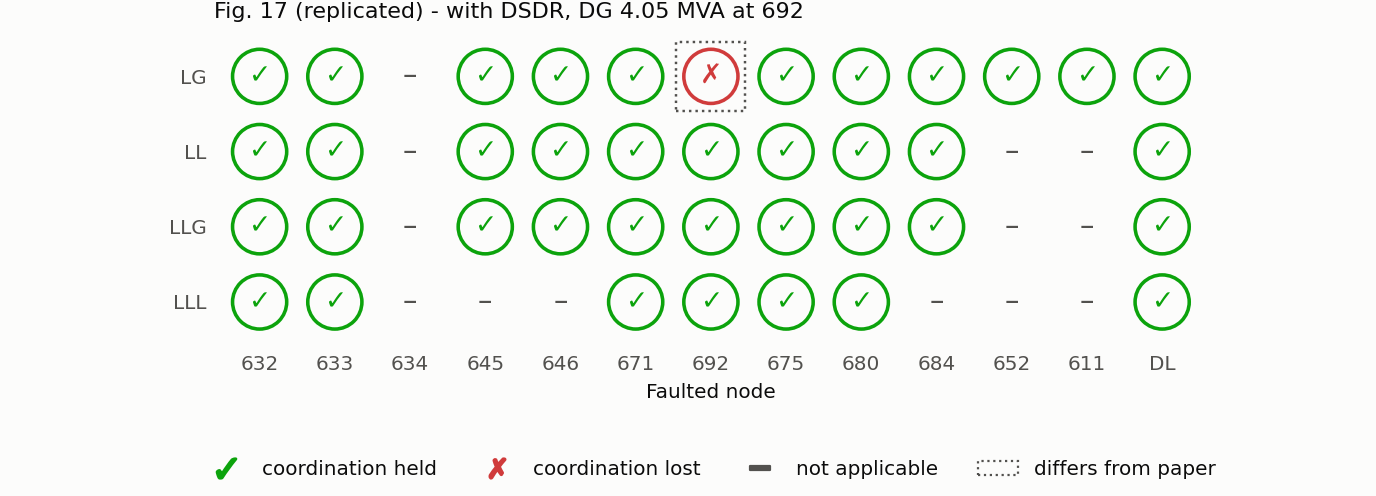
\includegraphics[width=0.9\textwidth]{fig17.png}
\caption{Coordination status with DG and the DSDR (replication of Fig.~17).}
\label{fig:f17}
\end{figure}

Figures~\ref{fig:f15} and \ref{fig:f16} show the paper's worked case, a bolted LL fault at 646. The fuses
carry 3.67\,kA (paper: 3.64\,kA). R2 carries 1.11\,kA in reverse (paper: 1.54\,kA) and trips on its reverse
fast curve in 0.086\,s (paper: 0.103\,s), before F646 melts.

\begin{figure}[H]
\centering
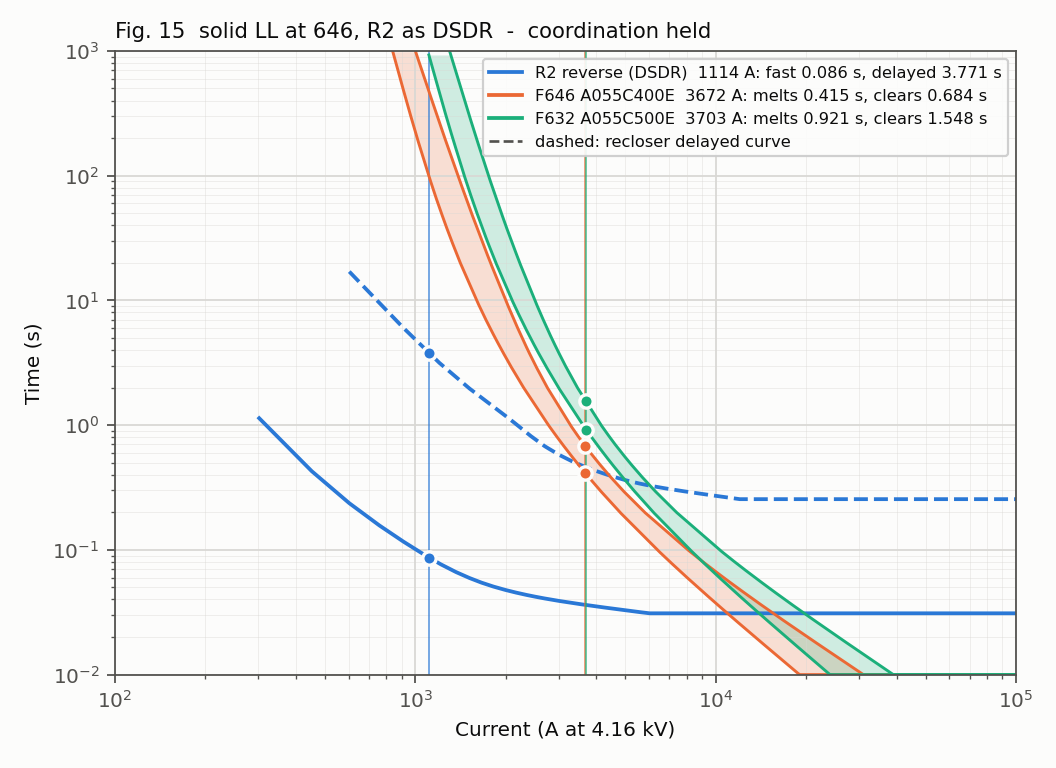
\includegraphics[width=0.68\textwidth]{fig15.png}
\caption{Bolted LL fault at 646: R2 reverse setting with F646 and F632 (Fig.~15 of the paper).}
\label{fig:f15}
\end{figure}

\begin{figure}[H]
\centering
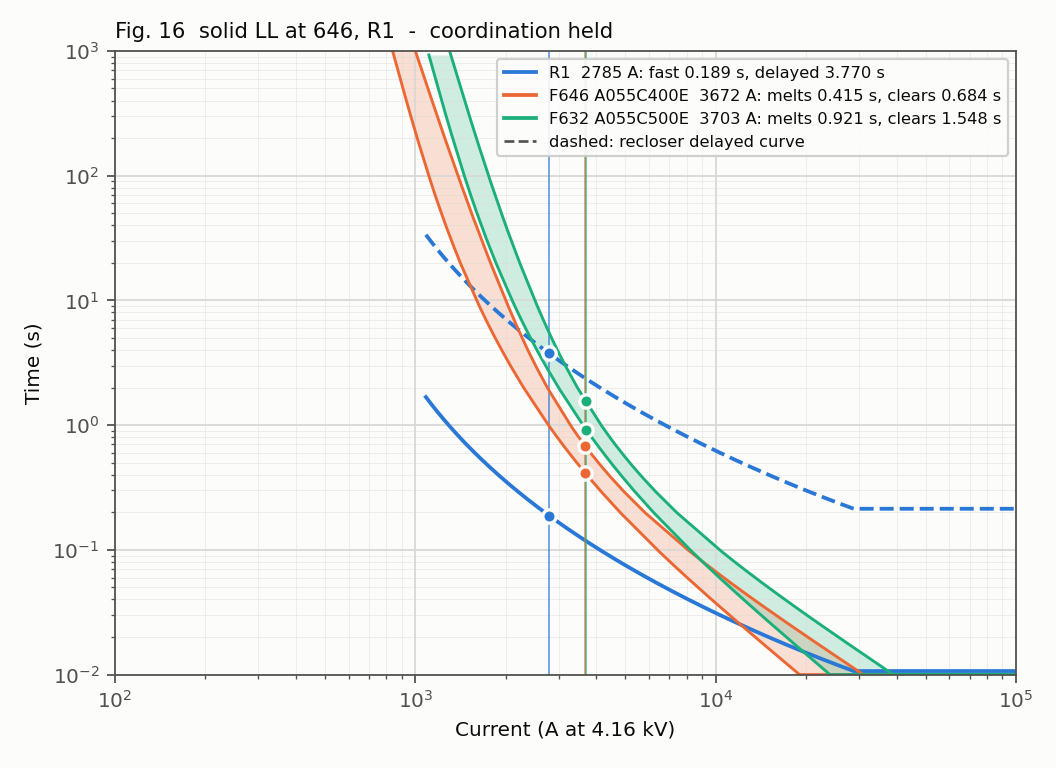
\includegraphics[width=0.68\textwidth]{fig16.png}
\caption{Bolted LL fault at 646: R1 with F646 and F632 (Fig.~16 of the paper).}
\label{fig:f16}
\end{figure}

\subsection{Operating Times With the DSDR (Table IV)}
Tables~\ref{tab:t4a} and \ref{tab:t4b} reproduce Table~IV of the paper. R1 operates forward for every node.
R2 operates in reverse for the nodes upstream of it and forward for the nodes downstream. The fuse time is
the minimum-melting time of the fuse nearest to the fault at the current through that fuse. In all nine
rows with a fuse it is longer than the last fast trip; the smallest margins are 6\,ms at 675 and 15\,ms at DL
and 652.

\begin{table}[H]
\centering\footnotesize
\setlength{\tabcolsep}{4pt}
\begin{tabular}{@{}llccccccc@{}}
\toprule
\hd & & \textbf{$I_{R1}$} & \textbf{R1 fast (s)} & \textbf{R1 delayed (s)} & \textbf{$I_{R2}$} & & \textbf{R2 fast (s)} & \textbf{R2 delayed (s)} \\
\hd\textbf{Node} & \textbf{Fault} & \textbf{(A)} & \textbf{model / paper} & \textbf{model / paper} & \textbf{(A)} & \textbf{Dir.} & \textbf{model / paper} & \textbf{model / paper} \\
\midrule
632 & LLL & 4734 & 0.081 / 0.070 & 1.627 / 1.398 & 1813 & rev & 0.051 / 0.045 & 1.416 / 0.514 \\
633 & LLL & 3970 & 0.106 / 0.094 & 2.111 / 1.880 & 1500 & rev & 0.060 / 0.052 & 2.001 / 0.706 \\
645 & LL & 3124 & 0.155 / 0.105 & 3.095 / 2.095 & 1232 & rev & 0.075 / 0.087 & 3.002 / 1.659 \\
646 & LL & 2785 & 0.189 / 0.128 & 3.770 / 2.555 & 1114 & rev & 0.086 / 0.103 & 3.771 / 2.046 \\
DL & LLL & 3954 & 0.106 / 0.087 & 2.123 / 1.733 & 1972 & rev & 0.048 / 0.076 & 1.213 / 1.402 \\
671 & LLL & 3412 & 0.134 / 0.105 & 2.677 / 2.091 & 3391 & fwd & 0.054 / 0.068 & 1.600 / 1.113 \\
692 & LLL & 3412 & 0.134 / 0.115 & 2.677 / 2.307 & 3391 & fwd & 0.054 / 0.072 & 1.600 / 1.258 \\
675 & LLL & 3090 & 0.158 / 0.121 & 3.152 / 2.414 & 3050 & fwd & 0.059 / 0.074 & 1.941 / 1.332 \\
684 & LL & 2543 & 0.222 / 0.125 & 4.437 / 2.507 & 2543 & fwd & 0.072 / 0.075 & 2.813 / 1.394 \\
680 & LLL & 2789 & 0.188 / 0.137 & 3.761 / 2.747 & 2757 & fwd & 0.066 / 0.079 & 2.381 / 1.555 \\
611 & LG & 1814 & 0.435 / 0.326 & 8.709 / 6.523 & 1718 & fwd & 0.128 / 0.146 & 6.986 / 4.385 \\
652 & LG & 1795 & 0.446 / 0.676 & 8.919 / 13.525 & 1761 & fwd & 0.123 / 0.143 & 6.570 / 9.370 \\
\bottomrule
\end{tabular}
\caption{Recloser operating times with the DSDR, DG in service (Table~IV of the paper).}
\label{tab:t4a}
\end{table}

\begin{table}[H]
\centering\footnotesize
\setlength{\tabcolsep}{4pt}
\begin{tabular}{@{}lllcccccccl@{}}
\toprule
\hd & & & & \textbf{$I_{fuse}$} & \multicolumn{2}{c}{\textbf{$t_{MMT}$ (s)}} & \textbf{$t_{TCT}$} & \textbf{Last fast} & \textbf{Margin} & \\
\hd\textbf{Node} & \textbf{Fault} & \textbf{Fuse} & \textbf{Size} & \textbf{(A)} & \textbf{model} & \textbf{paper} & \textbf{(s)} & \textbf{trip (s)} & \textbf{(s)} & \textbf{Status} \\
\midrule
633 & LLL & F633 & 400E & 5426 & 0.149 & 0.163 & 0.235 & 0.106 & $+0.043$ & held \\
645 & LL & F632 & 500E & 4191 & 0.613 & 0.276 & 0.970 & 0.155 & $+0.458$ & held \\
646 & LL & F646 & 400E & 3672 & 0.415 & 0.181 & 0.684 & 0.189 & $+0.226$ & held \\
DL & LLL & F-DL & 400E & 5902 & 0.121 & 0.248 & 0.193 & 0.106 & $+0.015$ & held \\
692 & LLL & F671-1 & 400E & 3391 & 0.525 & 0.175 & 0.891 & 0.054 & $+0.471$ & held \\
675 & LLL & F692-R & 250E & 5022 & 0.065 & 0.185 & 0.106 & 0.059 & $+0.006$ & held \\
684 & LL & F671-2 & 300E & 3963 & 0.148 & 0.205 & 0.230 & 0.072 & $+0.076$ & held \\
611 & LG & F684 & 200E & 2236 & 0.271 & 0.417 & 0.414 & 0.128 & $+0.143$ & held \\
652 & LG & F652 & 150E & 2239 & 0.138 & 0.233 & 0.193 & 0.123 & $+0.015$ & held \\
\bottomrule
\end{tabular}
\caption{Fuse times of Table~IV. Margin = $t_{MMT}$ minus the last fast trip (R2 for faults below R2; the later
of R1 and R2 reverse above it). Nodes 632, 671 and 680 are on the main feeder and have no fuse.}
\label{tab:t4b}
\end{table}

\subsection{Single Setting Against Dual Setting on Selected Faults}
Table~\ref{tab:cases9} compares the two settings of R2 on nine faults with the same (revised) fuses: the six
faults of the paper's figures and three cells of the classification. Figure~\ref{fig:cdsum} summarises it and
Figures~\ref{fig:case5} and \ref{fig:case7} show two of the diagrams.

\begin{table}[H]
\centering\scriptsize
\setlength{\tabcolsep}{3pt}
\begin{tabularx}{\textwidth}{@{}clLcccccccll@{}}
\toprule
\hd & \textbf{Paper} & & \textbf{$Z_f$} & \textbf{$I_{R1}$} & \textbf{$I_{R2}$ (A),} & \textbf{R1 fast} & \multicolumn{2}{c}{\textbf{R2 fast (s)}} & \textbf{Fuse: melts} & \multicolumn{2}{c}{\textbf{Fuse saving}} \\
\hd\textbf{\#} & \textbf{figure} & \textbf{Fault} & \textbf{($\Omega$)} & \textbf{(A)} & \textbf{direction} & \textbf{(s)} & \textbf{single} & \textbf{dual} & \textbf{(s)} & \textbf{single} & \textbf{dual} \\
\midrule
01 & Fig. 8 & LG fault at 611 & 0 & 1814 & 1718 (fwd) & 0.435 & 0.128 & 0.128 & F684 200E: 0.271 & held & held \\
02 & Fig. 9 & LLG fault at the middle of 692-675 & 1 & 1445 & 1310 (fwd) & 0.742 & 0.204 & 0.204 & F692-R 250E: 0.618 & held & held \\
03 & Fig. 11 & LL fault at 646 & 1 & 1899 & 847 (rev) & 0.395 & 0.500 & 0.131 & F646 400E: 1.734 & lost & lost \\
04 & Fig. 12 & LL fault at 645 & 1.5 & 1694 & 783 (rev) & 0.507 & 0.605 & 0.149 & F632 500E: 9.129 & lost & lost \\
05 & Fig. 13 & 3-phase fault at 10 \% of 632-633 & 0 & 4645 & 1777 (rev) & 0.084 & 0.121 & 0.052 & F633 400E: 0.100 & lost & held \\
06 & Figs. 15, 16 & LL fault at 646 & 0 & 2785 & 1114 (rev) & 0.189 & 0.278 & 0.086 & F646 400E: 0.415 & held & held \\
07 & Fig. 14 / 17 cell & LG fault at 646 (phase c) & 0 & 2359 & 469 (rev) & 0.255 & no trip & 0.396 & F646 400E: 1.057 & lost & held \\
08 & Fig. 14 / 17 cell & LG fault at 633 (phase b) & 0 & 2874 & 644 (rev) & 0.178 & 0.974 & 0.210 & F633 400E: 0.502 & lost & held \\
09 & Fig. 14 / 17 cell & LG fault at 692 (phase a) & 0 & 2197 & 2182 (fwd) & 0.293 & 0.089 & 0.089 & F671-1 400E: 2.842 & lost & lost \\
\bottomrule
\end{tabularx}
\caption{Nine faults with the DG in service: single-setting against dual-setting R2, same fuses.}
\label{tab:cases9}
\end{table}

In cases 5, 7 and 8 the dual setting restores the fuse saving: the reverse group picks up a DG current that
the forward group does not see (case 7: 469\,A) or sees only slowly. Cases 3, 4 and 9 are lost with both
settings; they are limits of the fuse revision and of the dial range, not of the direction. Cases 3 and 4 are
the paper's faults through impedance: the larger fuses that are needed for the bolted faults are too slow for
these lower currents.

\begin{figure}[H]
\centering
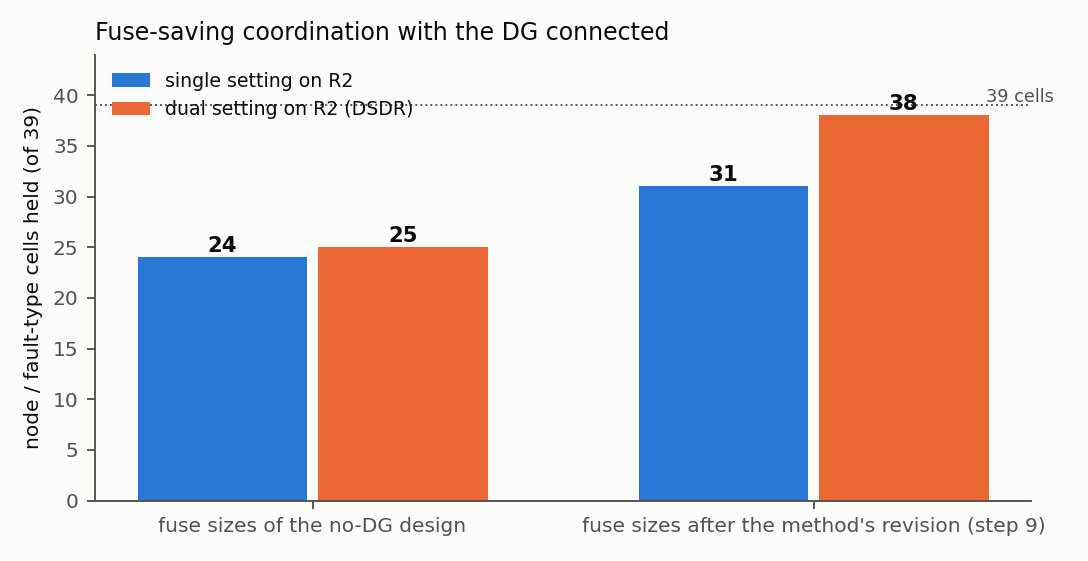
\includegraphics[width=\textwidth]{cd_summary.png}
\caption{Summary of the nine faults: single setting against dual setting.}
\label{fig:cdsum}
\end{figure}

\begin{figure}[H]
\centering
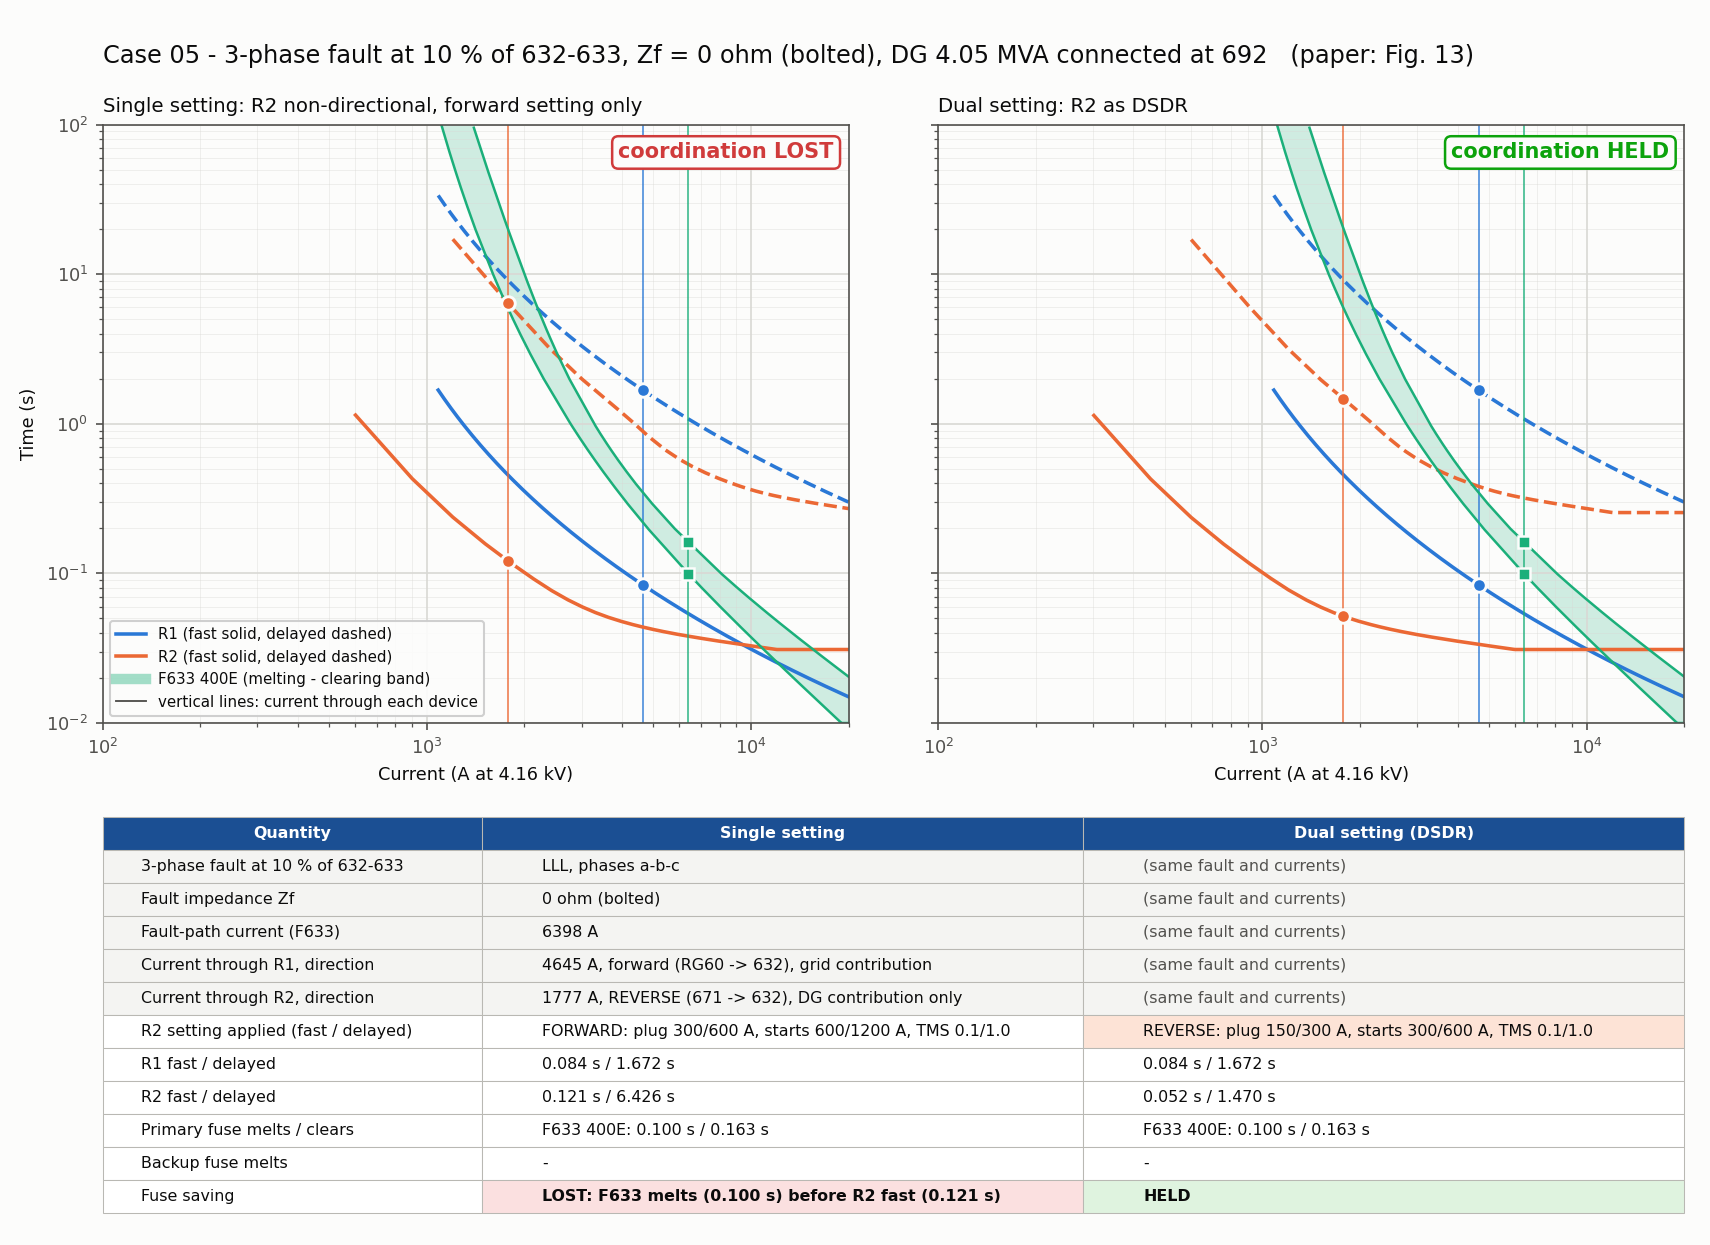
\includegraphics[width=\textwidth]{case05.png}
\caption{Three-phase fault at 10\,\% of line 632--633: single setting (left) and dual setting (right).}
\label{fig:case5}
\end{figure}

\begin{figure}[H]
\centering
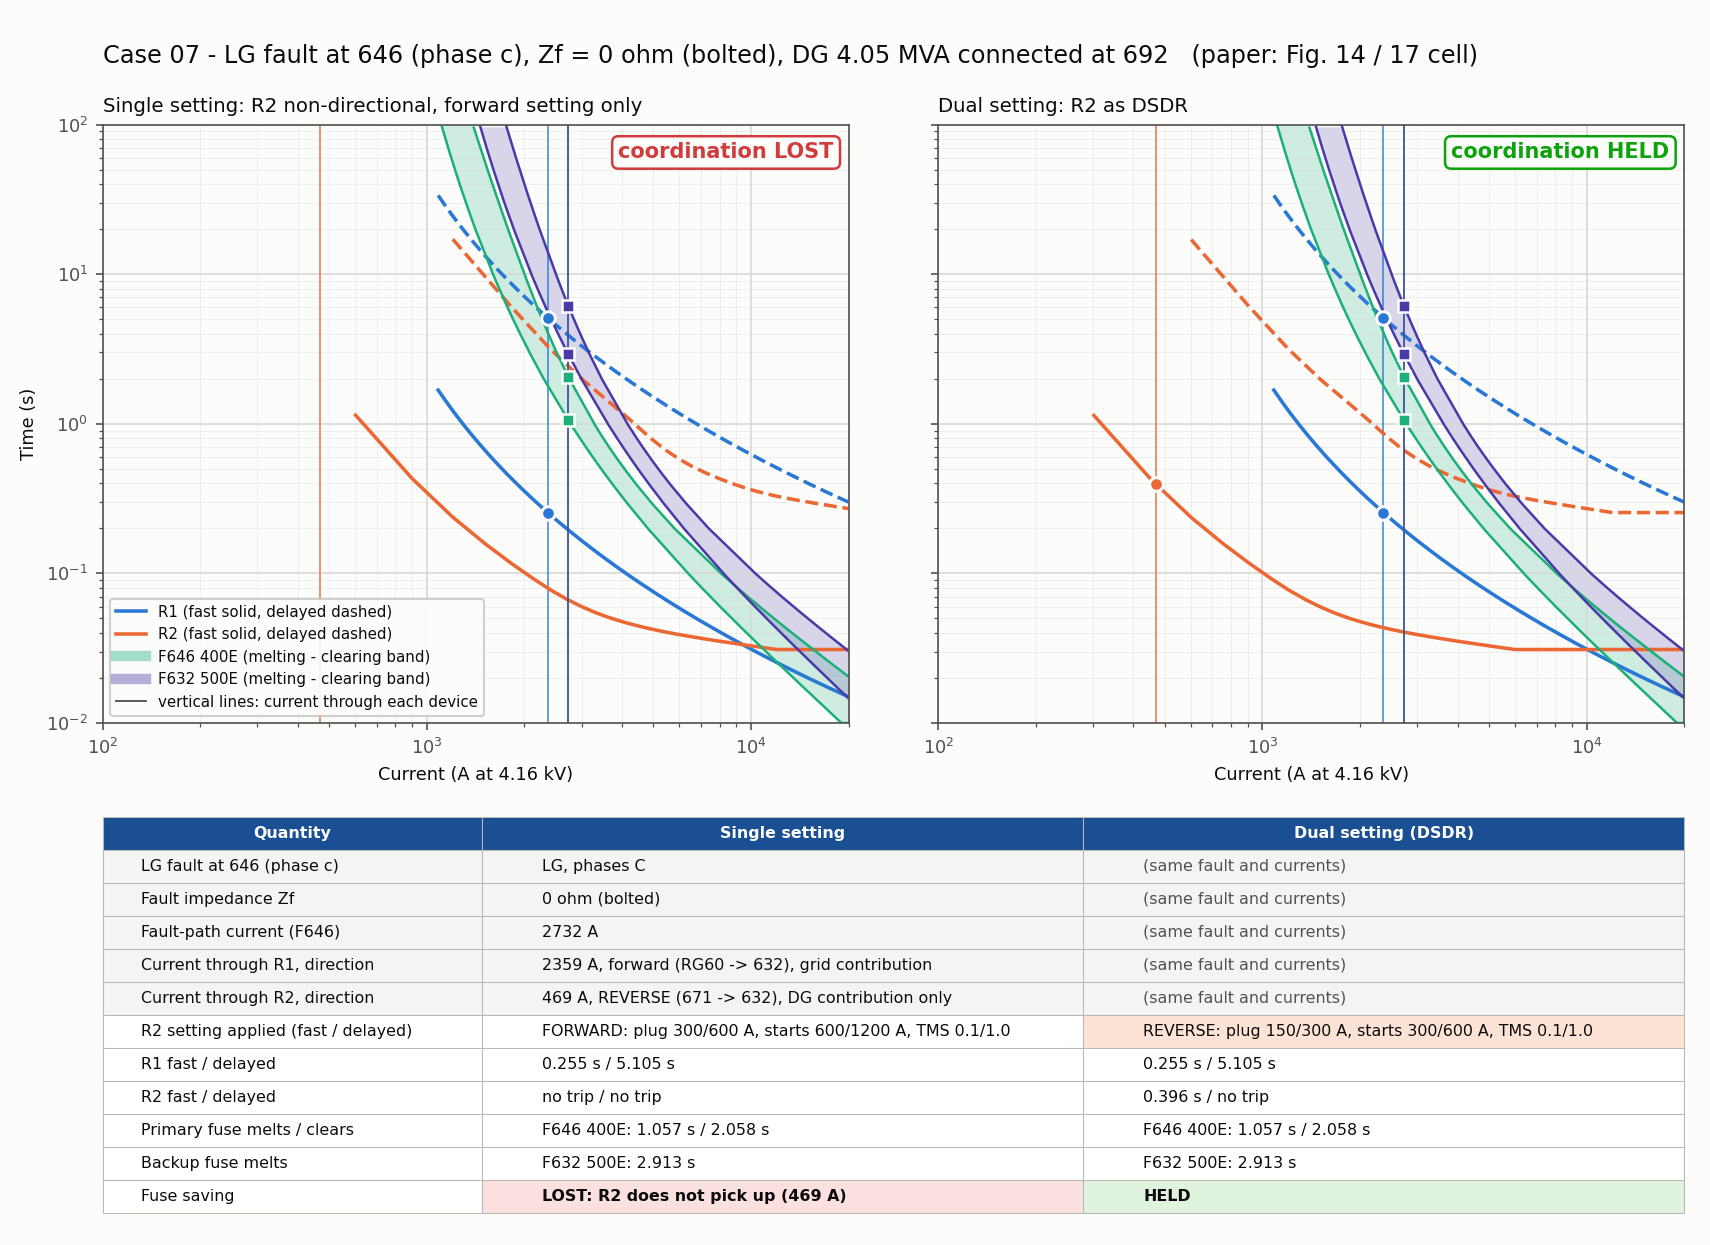
\includegraphics[width=\textwidth]{case07.png}
\caption{LG fault at 646: the single-setting R2 does not pick up the reverse current; the reverse group does.}
\label{fig:case7}
\end{figure}

\subsection{Time-Sequence Check}
The classification above uses the strict rule that every recloser must trip before the fuse starts to melt.
A time-sequence check follows each fault in time instead: the fuse heats with the current that still flows
after each recloser opens. For the 18 cells upstream of R2 the strict rule gives 11 cells held with the single
setting and 18 with the dual setting; the time sequence gives 15 and 18 (Figure~\ref{fig:seq}). The three
cells that the DSDR restores in the time sequence as well are the LG faults at 633, 645 and 646, where the
single-setting R2 never trips on a reverse current of about 0.5 to 0.6\,kA. For the 21 cells downstream of R2 the DG
at 692 feeds the fault directly, with no recloser in its path, and the result is the same for both settings.

\begin{figure}[H]
\centering
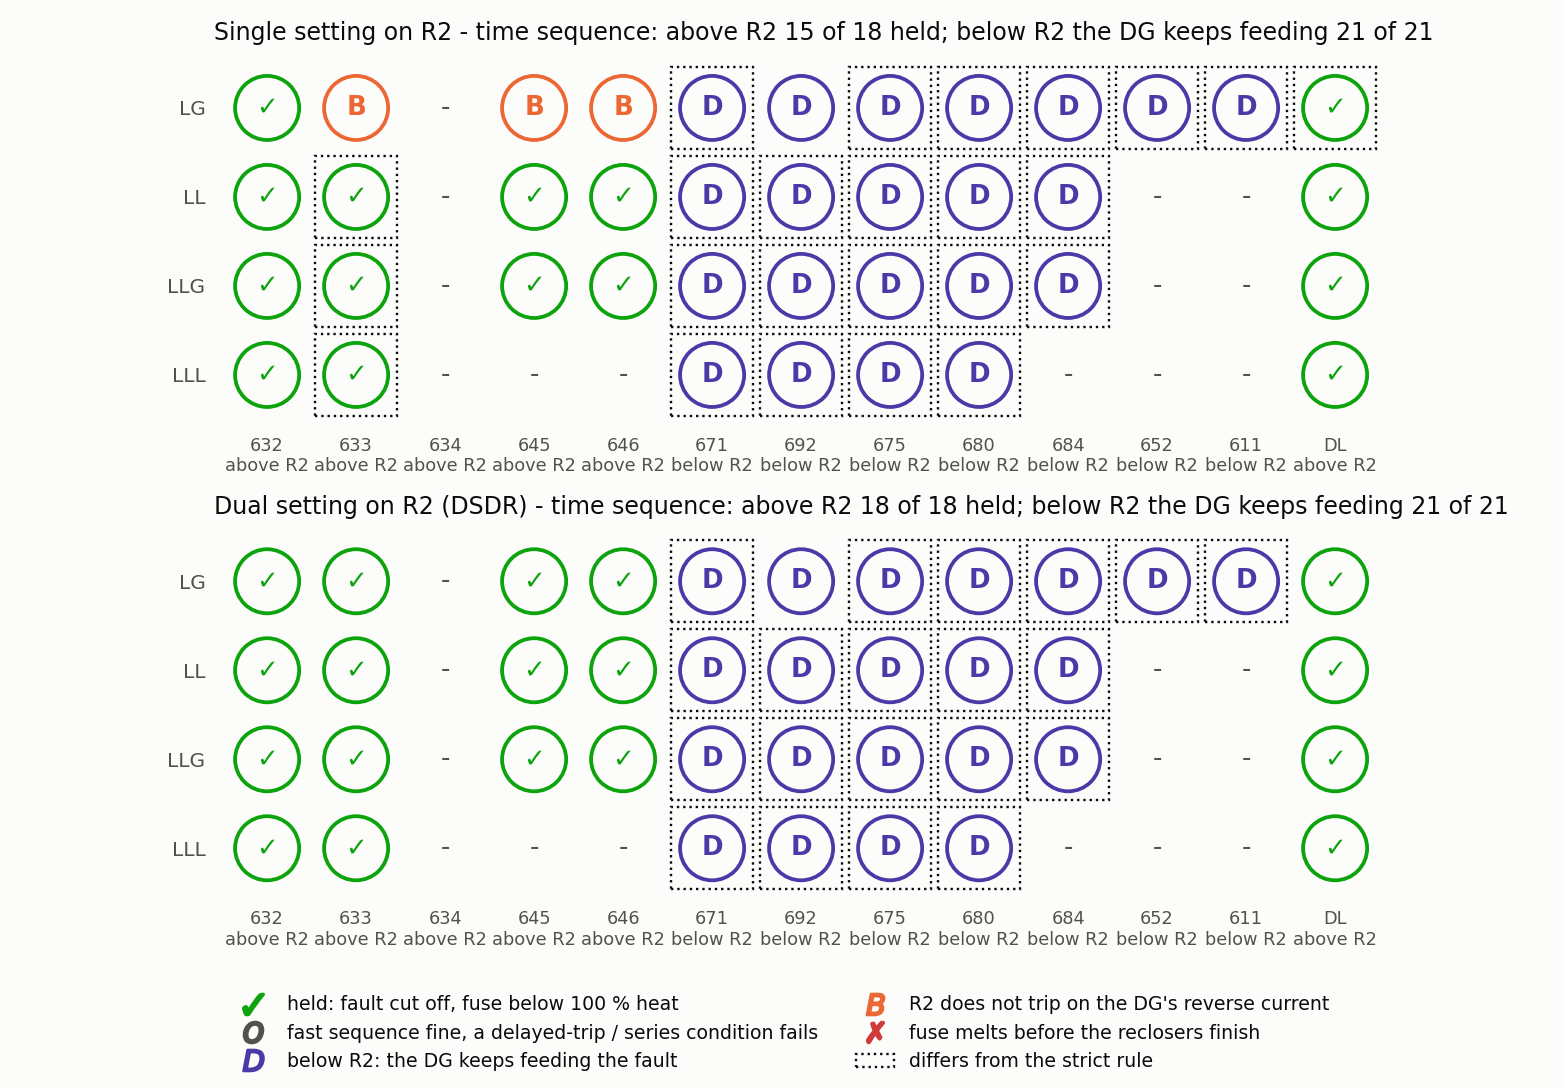
\includegraphics[width=\textwidth]{cd_sequence.png}
\caption{Time-sequence check of all 39 cells, single against dual setting.}
\label{fig:seq}
\end{figure}

\subsection{Time-Domain Verification (Fig. 10)}
Figure~\ref{fig:f10} is the EMT simulation of an LL (a--c) fault at 684 through 0.2\ohm{} with the
conventional settings. The recloser trips are scripted from R2's fast curve applied to the simulated current,
and the fuse F671-2 (300E) melts when the accumulated heating $\sum \Delta t / t_{MMT}(I)$ reaches one.
Without DG the two fast shots use 45\,\% of the melting heat, the fuse survives both and then clears the
permanent fault. With the DG the fuse melts at the end of the second fast shot, because the DG keeps feeding
the fault while R2 is open (Table~\ref{tab:emt}). The feeder current at node 632 is 557 / 588\,A RMS
(phases a / c) before the fault and 2362 / 2719\,A during it, with peaks of 3338 / 3842\,A; the paper's
larger phase peaks at about 5000\,A.

\begin{figure}[H]
\centering
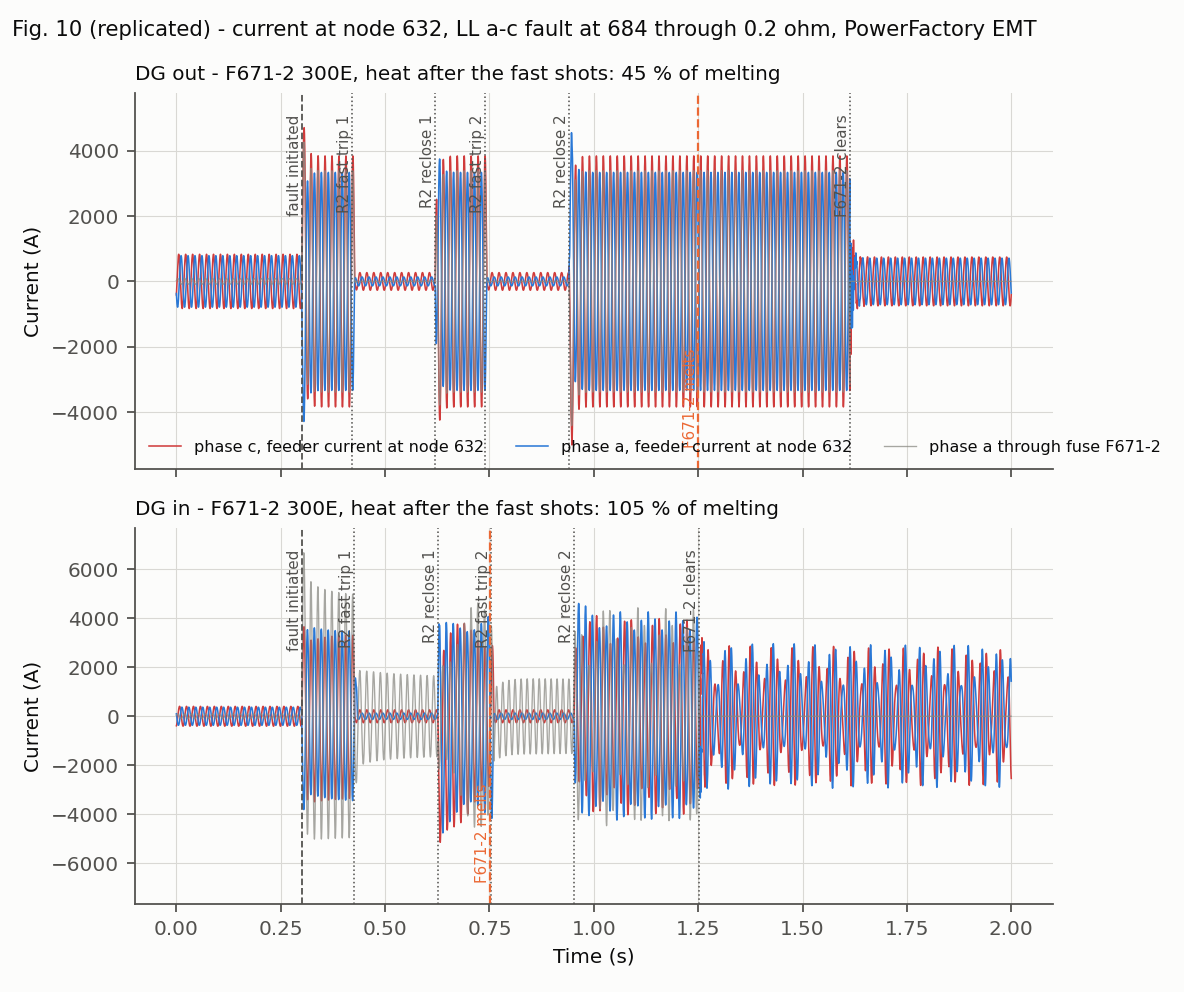
\includegraphics[width=0.95\textwidth]{fig10.png}
\caption{Time-domain current at node 632 for an LL (a--c) fault at 684 through 0.2\ohm{} (Fig.~10 of the paper):
without DG (top) and with DG (bottom).}
\label{fig:f10}
\end{figure}

\begin{table}[H]
\centering\small
\begin{tabular}{@{}lccc@{}}
\toprule
\hd\textbf{Event (time in s)} & \textbf{Paper (read off Fig.~10)} & \textbf{Model, DG out} & \textbf{Model, DG in} \\
\midrule
Fault initiated & 0.30 & 0.30 & 0.30 \\
R2 fast trip 1 & $\approx$0.46 & 0.420 & 0.426 \\
R2 reclose 1 & $\approx$0.65 & 0.620 & 0.626 \\
R2 fast trip 2 & $\approx$0.80 & 0.740 & 0.753 \\
R2 reclose 2 & $\approx$1.00 & 0.940 & 0.953 \\
Fuse F671-2 melts & -- & 1.248 & 0.752 \\
Fuse operation / clears & 1.21 & 1.613 & 1.253 \\
Fuse heat after the fast shots & -- & 45\,\% & 105\,\% \\
\bottomrule
\end{tabular}
\caption{Reclosing sequence of the EMT simulation against the paper.}
\label{tab:emt}
\end{table}

\subsection{Verification With the Relay and Fuse Models of \PF}
The operating times of Chapter Five are calculated in Python from the library curves. As a check, the
settings were written into the relay and fuse elements of the model, and \PF{} itself calculated the tripping
time of every device for every fault, for the conventional and for the DSDR settings. Over 1896 operating
times the largest deviation is 1.22\,\%.

\subsection{Sensitivity of the Result to the Margin}
\label{sec:margin}
The 38 held cells are obtained with a zero margin. If the breaker interrupting time of three cycles
is added to the fast trip, 31 cells are held; if in addition the fuse may only be loaded to 75\,\% of its
melting time, 26 cells are held. The pickups are a second limit: with the DG, the lowest LG fault current
through 3\ohm{} is 577\,A at R1 and 368\,A at R2, below the pickups of 734.6\,A and 587.5\,A, because the DG
supplies part of the fault. The paper examines neither point.

\subsection{Results Summary}
\begin{table}[H]
\centering\small
\begin{tabularx}{\textwidth}{@{}Lc@{}}
\toprule
\hd\textbf{Stage} & \textbf{Cells held (of 39)} \\
\midrule
A. No DG, starting fuse sizes & 35 \\
A. No DG, after the fuse revision (F692-R to 200E) & 39 \\
B. DG connected, conventional R2 (Fig.~14) & 24 \\
B. DG connected, no-DG fuses, R2 as DSDR & 25 \\
C. DG connected, revised fuses, conventional R2 & 31 \\
C. DG connected, revised fuses, R2 as DSDR (Fig.~17) & 38 \\
C. The same settings and fuses with the DG out of service & 37 \\
\bottomrule
\end{tabularx}
\caption{Summary of the coordination results.}
\label{tab:summary}
\end{table}

The dual setting alone, with the fuses of the design without DG, restores one cell (24 to 25). Together with
the fuse revision it restores fourteen (24 to 38), seven of which need the dual setting.

% =====================================================================================================
\chapterhead{SIX}{COMPARISON OF RESULTS WITH THE REFERENCE PAPER}

\subsection{Basis of Comparison}
The comparison uses only values that the paper prints or that can be read from its figures. The model was
not tuned to match the paper; differences are stated and explained from the evidence in the model.

\begin{table}[H]
\centering\footnotesize
\begin{tabularx}{\textwidth}{@{}LLLl@{}}
\toprule
\hd\textbf{Aspect} & \textbf{This project} & \textbf{Reference paper} & \textbf{Assessment} \\
\midrule
Rated branch currents & within 2\,\% & Table II & Very good \\
Fault levels & IEEE benchmark, feeder head 4.73\,kA & 5.41\,kA, some branches higher & Lower \\
R1 worked example (4219\,A) & 0.096 / 1.926\,s & 0.097 / 1.932\,s & Very good \\
Recloser curves & IAC77B801A and CDG34 library curves & Same devices & Same \\
Fuse coefficients, series fuses of R1's zone & within 0.05 with reversed index & Table III & Index reversed in the paper \\
DG model & Dynamic synchronous machine, Table I data & Synchronous machine & Same \\
Coordination with DG, conventional R2 & 24 of 39 held; 29 cells agree & 30 of 39 held (Fig.~14) & Good \\
Coordination with the DSDR & 38 of 39 held & 39 of 39 held (Fig.~17) & Good; one cell at the dial limit \\
Fuse current, LL at 646 & 3.67\,kA & 3.64\,kA (Fig.~15) & Very good \\
R2 reverse current, LL at 646 & 1.11\,kA & 1.54\,kA & Lower \\
Table IV, R1 times & 12 to 78\,\% slower (652: 34\,\% faster) & Table IV & Follows the fault levels \\
Table IV, R2 and fuse times & assumed R2 settings, revised fuses & settings not published & Not comparable in detail \\
EMT sequence, fuse operation & melts 1.25\,s, clears 1.61\,s & 1.21\,s (Fig.~10) & Close if 1.21\,s is melting \\
IEEE 34-node feeder & not modelled & validated & Remaining work \\
\bottomrule
\end{tabularx}
\caption{Comparison of the results with the reference paper.}
\label{tab:compare}
\end{table}

\subsection{Base-Case Comparison}
The rated currents test the feeder model independently of the protection and of the DG. Their agreement
within 2\,\% (the MATLAB/Simulink model of the earlier phase reached 2 to 9\,\%) shows that the topology, the
loads and the regulator are implemented as in the paper.

\subsection{Fault-Current Magnitude Difference}
The maximum fault currents of the feeder branches are 4 to 60\,\% below the paper's Table~II. The model was validated against the
published IEEE short-circuit results instead, which it meets within about 2\,\%. The paper's values cannot
all be correct: 6.73\,kA on 632--633 and 7.83\,kA on 692--675 exceed its own 5.41\,kA at the feeder head. The
two worked cases of the paper illustrate the remaining difference: R2 carries 1718\,A for the LG fault at
611 (paper: 1974\,A) and 1114\,A in reverse for the LL fault at 646 (paper: 1542\,A). In the earlier
MATLAB/Simulink phase these currents were 702\,A and 838\,A, because the DG was a static Thevenin source.

\subsection{Fuse and Coordination Comparison}
The paper's Table~III could be reproduced only with the series index reversed. The fuse times in the paper's
figures do not follow its fuse equation: for F646 at 3.6\,kA the figure shows about 0.18\,s, the equation
with Table~III gives 1.85\,s. The figures match A055C library fuses, and the sizes change between figures
(F646 is 200E in Fig.~12 and 300E in Figs.~11 and 16). The model therefore uses library fuse curves
throughout.

\subsection{Operating-Time Comparison (Table IV)}
The R1 equation and settings reproduce the paper's worked example, so the difference of the R1 times comes
from the fault currents. In every row of the paper the delayed time of R1 is 20 times the fast time, the
ratio of the dials 10 and 0.5, which confirms the dials. For R2 the paper prints no settings and the ratio of
its two times is not constant, so the R2 times and the fuse times of the model are the result of the stated
method and cannot be matched to the paper row by row.

\subsection{Central Finding Comparison}
The central finding of the paper is reproduced: the DG makes a conventional scheme lose coordination in the
zone between the grid and the DG, and a dual-setting directional R2 restores it there. The model adds two
qualifications. The dual setting needs the fuse revision to be effective; and it does not help for faults
downstream of R2, which the DG feeds directly.

% =====================================================================================================
\chapterhead{SEVEN}{DISCUSSION}

\subsection{Effect of DG on Fault Current}
The DG raises the fault current at every node, most near its connection point (671 and 692: from 3.39 to
5.56\,kA). The fuses carry this higher current and melt faster, while R1 carries about the same grid current
as before. The margin between the fuse and the fast trip, which is small even without DG, disappears.

\subsection{Effect of Fault Current Direction}
For faults at 632, 633, 645, 646 and DL the current through R2 is reverse and consists only of the DG
contribution. Its magnitude (0.5 to 2.0\,kA) is much lower than the forward fault currents for which the
forward group is set. A forward group with plugs of 300 and 600\,A responds slowly to these currents, or not
at all for LG faults.

\subsection{Performance of the Conventional Protection}
With the conventional single setting the scheme keeps coordination at the nodes on the main feeder and loses
it on the fused laterals of R1's zone and at 675. The loss depends on the location and on the fault type; it
is not a uniform failure of the feeder.

\subsection{Performance of the DSDR}
The reverse group, with half the plug settings, trips for every reverse fault before the fuse melts once the
fuses are revised. The result of 38 cells against 31 with the same fuses isolates its contribution. Without
the fuse revision the improvement is one cell only: at 633 and DL the fuses of the design without DG melt
in 0.05 to 0.16\,s with the DG, before R1's fast trip (0.11 to 0.18\,s), and no setting of R2 can change
R1's time. The
DSDR is therefore necessary but not sufficient.

\subsection{Limits Reached by the Devices}
R1's dials in the paper are the two extremes of the IAC range, and the CDG table ends at 0.1 and 1.0. The
method's dial revision has no room. The fuse revision creates a conflict between the two states of the
network: the larger fuses that are needed with the DG are too slow for two cells without it, and for the
paper's impedance faults. Fuse sizes cannot adapt to the DG state. For faults downstream of R2 the fuse
saving relies on the DG's own protection disconnecting it during the dead time, which the paper does not
treat.

\subsection{Change of the Simulation Tool}
Rebuilding the study in \PF{} removed the main limitations of the earlier MATLAB\slash Simulink phase. The DG is a
dynamic synchronous machine with the full data of the paper instead of a static source. The reclosers use
the curves of the devices named in the paper instead of a substitute curve. All 39 cells are
resolved, including the three-phase faults and the single-phase nodes that could not be built before. The
complete DSDR stage, which was pending, is finished. The earlier model remains useful as an independent
cross-check of the load flow.

\subsection{Engineering Implication}
Adaptive directional protection is justified where a DG is downstream of a mid-line recloser. To apply it,
the engineer must check the dial range of the actual relay, revise the fuse sizes for the DG state, verify the
pickup against the reduced minimum fault current with DG, and provide for the DG infeed to faults beyond the
recloser.

% =====================================================================================================
\chapterhead{EIGHT}{CONCLUSION AND FUTURE WORK}

\subsection{Conclusion}
The DSDR method of Yousaf \textit{et al.} was implemented on the IEEE 13-node feeder in DIgSILENT \PF{} with
the real characteristics of the devices named in the paper. The feeder model agrees with the paper's rated
currents within 2\,\% and with the IEEE short-circuit benchmark within about 2\,\%. Without DG the
conventional scheme is coordinated in all 39 cells. With the 4.05\,MVA DG at node 692 and a
conventional R2, coordination is held in 24 cells. With R2 as a DSDR and the fuse revision of the
method it is held in 38 cells; with the same fuses and a single setting in 31. The
central finding of the paper is therefore confirmed, with the qualification that the result depends on the
fuse revision and that one cell and the faults downstream of R2 remain open.

\subsection{Major Findings}
\begin{enumerate}
\item Rated currents within 2\,\% of the paper; fault levels at the IEEE benchmark, lower than the paper's.
\item R1: pickup 720\,A, TDS 0.5 / 10; the IAC equation reproduces the paper's worked example within 1\,\%.
\item R2 forward: plugs 300 / 600\,A, TMS 0.1 / 1.0; R2 reverse: plugs 150 / 300\,A, TMS 0.1 / 1.0; reverse
      pickup by eq.~(12) 315.3\,A.
\item With DG the load current at R2 reverses (252\,A) and R2 carries 1.1 to 2.0\,kA in reverse for upstream
      faults.
\item Coordination: 39 cells without DG; 24 with DG and a conventional R2; 38 with the
      DSDR; 29 cells agree with the paper's Fig.~14.
\item The dual setting restores seven cells with the revised fuses and one cell without the revision.
\item The LG fault at 692 cannot be coordinated within the dial range of R2.
\item \PF's own relay and fuse models confirm the operating times within 1.22\,\%.
\item In the EMT simulation the fuse survives the two fast shots without DG and melts at 1.25\,s (paper:
      fuse operation at 1.21\,s); with DG it melts during the second fast shot.
\end{enumerate}

\subsection{Contributions of the Present Work}
\begin{itemize}
\item A reproducible \PF{} implementation of the method: one command rebuilds the model and all results.
\item Separation of the effect of the dual setting from the effect of the fuse revision.
\item Identification of inconsistencies in the reference paper: the reversed index in Table~III, fuse curves
      in the figures that differ from the fuse equation, fuse sizes that change between figures, and fault
      levels above the feeder-head value.
\item Identification of the limits of the method: dial range, DG-in against DG-out fuse sizes, DG infeed
      downstream of the recloser, and sensitivity of the pickups with DG.
\item A time-domain verification and a verification with the relay models of the tool.
\end{itemize}

\subsection{Remaining Work}
\begin{enumerate}
\item Extend the study to the IEEE 34-node feeder (Figs.~18 to 20 and Table~V of the paper).
\item Model the directional element of R2 explicitly instead of assigning the direction from the fault location.
\item Repeat the classification with a practical margin (breaker time and 75\,\% of the fuse melting time).
\end{enumerate}

\subsection{Future Work}
Future work may include a recloser with a wider dial range or with user-defined curves, a setting-group
change triggered by the DG state, the disconnection logic of the DG during the reclosing dead time, the
sensitivity to fault impedance, inverter-based generation, and hardware-in-the-loop tests.

% =====================================================================================================
\clearpage
\phantomsection\addcontentsline{toc}{section}{REFERENCES}
\begin{thebibliography}{9}
\bibitem{yousaf2022} M.~Yousaf, A.~Jalilian, K.~M.~Muttaqi, and D.~Sutanto, ``An adaptive overcurrent
protection scheme for dual-setting directional recloser and fuse coordination in unbalanced distribution
networks with distributed generation,'' \textit{IEEE Transactions on Industry Applications}, vol.~58, no.~2,
pp.~1831--1842, Mar./Apr.\ 2022, doi: 10.1109/TIA.2022.3146095.
\bibitem{kersting1991} W.~H.~Kersting, ``Radial distribution test feeders,'' \textit{IEEE Transactions on
Power Systems}, vol.~6, no.~3, pp.~975--985, Aug.\ 1991.
\bibitem{benmouyal1999} G.~Benmouyal \textit{et al.}, ``IEEE standard inverse-time characteristic equations
for overcurrent relays,'' \textit{IEEE Transactions on Power Delivery}, vol.~14, no.~3, pp.~868--872,
Jul.\ 1999.
\bibitem{naiem2012} A.~Naiem, Y.~Hegazy, A.~Abdelaziz, and M.~Elsharkawy, ``A classification technique for
recloser-fuse coordination in distribution systems with distributed generation,'' \textit{IEEE Transactions
on Power Delivery}, vol.~27, no.~1, pp.~176--185, Jan.\ 2012.
\bibitem{yousaf2020} M.~Yousaf, K.~M.~Muttaqi, and D.~Sutanto, ``Overcurrent protection scheme for the IEEE
13-node benchmark test feeder with improved selectivity,'' in \textit{Proc.\ IEEE Power \& Energy Society
General Meeting}, 2020, doi: 10.1109/PESGM41954.2020.9281529.
\bibitem{kersting2012} W.~H.~Kersting and G.~Shirek, ``Short circuit analysis of IEEE test feeders,'' in
\textit{Proc.\ IEEE PES Transmission and Distribution Conference and Exposition}, 2012.
\bibitem{pf2021} DIgSILENT GmbH, \textit{PowerFactory 2021 User Manual}, Gomaringen, Germany, 2021.
\end{thebibliography}

% =====================================================================================================
\appendixhead{A}{COMPLETE COPY OF THE REFERENCE PAPER}
The complete reference paper by Yousaf \textit{et al.}~\cite{yousaf2022} is attached as a separate, unchanged
PDF copy in accordance with the requirement of the department. It is not reproduced inside this document.

\appendixhead{B}{POWERFACTORY MODEL AND PARAMETER NOTES}
\begin{itemize}
\item Project: \emph{IEEE13 Yousaf2022 Replication}, imported from \texttt{IEEE 13 Node Feeder.pfd}; study
      case \emph{Study with Substation Transformer}.
\item Source: external grid 115\,kV, substation transformer 115/4.16\,kV, 5\,MVA, $u_k = 8.06\,\%$.
\item Regulator taps fixed at +10 (a), +8 (b), +11 (c).
\item DG: synchronous machine 4.05\,MVA, 0.69\,kV, round rotor, data of Table~\ref{tab:dg}; transformer
      4.16/0.69\,kV, $u_k = 15\,\%$; operating point 3.24\,MW, voltage control at 1.0\,p.u.
\item R1: relay type IAC77B801A at RG60--632, units ``R1 Fast'' and ``R1 Delayed''.
\item R2: relay type CDG34 at the 671 end of line 632--671, units ``R2 Fast'', ``R2 Delayed'', ``R2 Rev Fast''
      and ``R2 Rev Delayed''.
\item Fuses: fuse elements with the library types A055C (4.16\,kV) and gL-800A (0.48\,kV).
\item The protection devices are created in the base network. Changes made while the substation-transformer
      variation is active are recorded in that variation and are removed by the scripts after each run.
\item \PF{} must be closed when the scripts are run from Python; inside \PF{} the script object
      \texttt{Final(1)} runs the same sequence.
\end{itemize}

\appendixhead{C}{IMPLEMENTATION FORMULAS}
The operating times are evaluated with the following expressions, where $M = I_f/I_p$ for R1 and
$M = I_f/I_s$ for R2.
\begin{align}
\text{R1 (IAC):}\quad & t = TDS\left[0.004+\frac{0.6379}{M-0.62}+\frac{1.7872}{(M-0.62)^2}+\frac{0.2461}{(M-0.62)^3}\right] \tag{A}\\
\text{R2 (CDG table):}\quad & t = t_1\left(\frac{t_2}{t_1}\right)^{f},\quad f=\frac{\ln(M/M_1)}{\ln(M_2/M_1)} \tag{B}\\
\text{Fuse (curve points):}\quad & t = t_1\left(\frac{t_2}{t_1}\right)^{f},\quad f=\frac{\ln(I/I_1)}{\ln(I_2/I_1)} \tag{C}\\
\text{Fuse saving:}\quad & t_{MMT}(I_{fuse}) > t_F ,\qquad t_{TCT}(I_{fuse}) < t_D \tag{D}\\
\text{Series fuses:}\quad & t_{TCT,\,i} \le 0.75\,t_{MMT,\,i+1} \tag{E}\\
\text{Fuse heating (EMT):}\quad & \sum_j \frac{\Delta t_j}{t_{MMT}(I_j)} = 1 \;\Rightarrow\; \text{the fuse melts} \tag{F}
\end{align}

\textbf{Worked example, node 633, three-phase fault, DG in service.} R1 carries 3970\,A:
$M = 3970/720 = 5.514$, $M-0.62 = 4.894$, bracket $= 0.004+0.1303+0.0746+0.0021 = 0.2111$, so
$t_F = 0.5\times0.2111 = 0.106$\,s and $t_D = 10\times0.2111 = 2.111$\,s. R2 carries 1500\,A in reverse:
fast, $M = 1500/150 = 10.0$, table 0.060\,s; delayed, $M = 1500/300 = 5.0$, table 2.0\,s. The fuse F633 (400E)
carries 5426\,A, the sum of both contributions: its curve points are 4800\,A at 0.2\,s and 6392\,A at 0.1\,s,
$f = \ln(5426/4800)/\ln(6392/4800) = 0.428$, $t_{MMT} = 0.2\times0.5^{0.428} = 0.149$\,s. The fuse outlasts the
last fast trip (0.106\,s) by 0.043\,s.

\appendixhead{D}{CURRENT PROJECT STATUS}
\begin{table}[H]
\centering\small
\begin{tabularx}{\textwidth}{@{}LlL@{}}
\toprule
\hd\textbf{Work package} & \textbf{Status} & \textbf{Evidence} \\
\midrule
IEEE 13-node model in \PF & Completed & Rated currents within 2\,\%, fault levels at the IEEE benchmark \\
Unbalanced load flow & Completed & Tables~\ref{tab:volt} and \ref{tab:lf} \\
Short-circuit analysis & Completed & All fault types and phase combinations, DG out and in \\
DG connection (dynamic machine) & Completed & Table~\ref{tab:dg} \\
Conventional coordination without DG & Completed & 39 of 39 cells \\
Classification with DG (Fig.~14) & Completed & 24 of 39 cells held, 29 agree with the paper \\
DSDR forward and reverse settings & Completed & Table~\ref{tab:settings} \\
DSDR coordination restoration (Fig.~17, Table~IV) & Completed & 38 of 39 cells \\
Time-domain verification (Fig.~10) & Completed & Table~\ref{tab:emt} \\
Verification with \PF{} relay models & Completed & 1896 operating times, max 1.22\,\% \\
CTI against DG penetration (Fig.~7) & Not included & Quantity not defined in the paper \\
IEEE 34-node extension & Pending & Not started \\
\bottomrule
\end{tabularx}
\caption{Status of the work packages.}
\label{tab:status}
\end{table}

\end{document}
